\documentclass[12pt]{article}
%\usepackage[T1]{fontenc}
\usepackage[utf8]{inputenc}

\usepackage{ifpdf}
\usepackage{listings}
\usepackage[small,bf]{caption}
\usepackage[titletoc]{appendix}
\usepackage{endnotes}
\renewcommand*{\thefootnote}{\fnsymbol{footnote}}
%\usepackage{marginnote} %ääremärkuste tegemiseks

\usepackage[margin=3cm]{geometry}


\usepackage{subfig}
\usepackage[final]{graphicx}
\usepackage{lineno}

\usepackage{fancyhdr}
\usepackage{amsmath}
\usepackage[acronym]{glossaries} %abbreviations
\usepackage{subfloat}

\usepackage{amssymb}
\usepackage{cancel}

\usepackage{hyperref} %klikitavad lingid
\usepackage{cleveref}

\usepackage[
    hyperref=true,
    url=false,
    isbn=false,
    backref=true,
    style=numeric-comp,
    block=none
]{biblatex}
\bibliography{bibliography}

\hypersetup{colorlinks=true, linktoc=page}

%\topmargin -1.5cm
% \oddsidemargin -0.1cm
% \evensidemargin -0.1cm
% \textwidth 16.59cm
% \textheight 21.94cm
%\pagestyle{fancyplain}
\linespread{1.5}
\parindent 0.5cm


\usepackage{multirow,bigdelim} %tabelisse veergude-ridade ühendamine

%iga uus sektsioon algab uuelt lehelt
\let\stdsection\section

%\usepackage[toc,nonumberlist,acronym]{glossaries}

\newcommand{\ttbar}{\ensuremath{\mathrm{t} \bar{\mathrm{t}}}}
\newcommand{\ttH}{\ensuremath{\mathrm{t} \bar{\mathrm{t}} \mathrm{H}}}
\newcommand{\ttHbb}{\ensuremath{\mathrm{t} \bar{\mathrm{t}} \mathrm{H} (\rightarrow \mathrm{b}\bar{\mathrm{b}})}}
\newcommand{\Hbb}{\ensuremath{\mathrm{H} \rightarrow \mathrm{b}\bar{\mathrm{b}}}}
\newcommand{\ttHnonbb}{\ensuremath{\mathrm{t} \bar{\mathrm{t}} \mathrm{H} (\rightarrow \mathrm{non}~\mathrm{b}\bar{\mathrm{b}})}}
\newcommand{\ttbb}{\ensuremath{\mathrm{t} \bar{\mathrm{t}} + \mathrm{b}\bar{\mathrm{b}}}}
\newcommand{\ttcc}{\ensuremath{\mathrm{t} \bar{\mathrm{t}} + \mathrm{c}\bar{\mathrm{c}}}}
\newcommand{\ttb}{\ensuremath{\mathrm{t} \bar{\mathrm{t}} + \mathrm{b}}}
\newcommand{\tttwob}{\ensuremath{\mathrm{t} \bar{\mathrm{t}} + 2\mathrm{b}}}
\newcommand{\ttlf}{\ensuremath{\mathrm{t} \bar{\mathrm{t}} + \mathrm{LF}}}
\newcommand{\bb}{\ensuremath{\mathrm{b}\bar{\mathrm{b}}}}
\newcommand{\fix}{~\textbf{FIXME}~}
\newcommand{\GeV}{\ensuremath{~\mathrm{GeV}}}
\newcommand{\TeV}{\ensuremath{~\mathrm{TeV}}}
\newcommand{\MET}{\ensuremath{\mathrm{MET}}}
\newcommand{\ptgen}{\ensuremath{p_{T,\mathrm{gen}}}}
\newcommand{\ifb}{\ensuremath{\mathrm{fb}^{-1}}}
\newcommand{\madgraphatnlo}{\verb+MG5_aMC@NLO+}
\newcommand{\powheg}{\texttt{POWHEG}}
\newcommand{\pythia}{\texttt{Pythia}}
\newcommand{\herwig}{\texttt{HERWIG++}}
\newcommand{\geant}{\texttt{GEANT4}}
\renewcommand{\vec}[1]{\boldsymbol{#1}}

\begin{document}
%\selectlanguage{english}
\linenumbers

\section{Introduction}

\section{Matrix Element Method}
\label{sec:mem}

\subsection{Hypothesis testing}

\subsection{Optimal test statistic}
\label{sec:test_statistic}

\subsection{Description of MEM}

The MEM is a multivariate analysis technique in which we directly compute the per-event probability density that depends on model parameters $\vec{\theta}$

\begin{equation}
P_{\vec{\theta}}(\vec{y}) = \frac{1}{\sigma}
\frac{\mathrm{d}\sigma_{\vec{\theta}}(\vec{y})}{\mathrm{d}\vec{y}}
\end{equation}
and use it in hypothesis testing as component of the test statistic. Through the differential cross section, the MEM explicitly depends on $\vec{y} = (\tilde{p}_{i \in \mathrm{jets}}, \tilde{p}_{i \in \mathrm{leptons}}, \dots)$, the vector containing the detector-level 4-momenta of the reconstructed particles, in particular, jets and leptons. The differential cross-section(\cref{eq:diff_cross_section}) depends on the squared matrix element $|\mathcal{M}^2|$ that we use to directly take into account the dynamics of the relevant underlying processes. The kinematics of the $2 \rightarrow n$ scattering process are encoded in the $n$-body phase space element(\cref{eq:n_body_phase_space}), where the delta function enforces the conservation of momentum between the initial and final state particles.

\begin{equation}
\label{eq:diff_cross_section}
\mathrm{d}\sigma_{\vec{\theta}} = \frac{(2\pi)^4 |\mathcal{M}_{\vec{\theta}}|^2}{4 \sqrt{(q_1 \cdot q_2)^2 - m_1 m_2}} \times
\mathrm{d}\Phi_n(q_1 + q_2; p_1, \dots, p_{n})
\end{equation}

\begin{equation}
\label{eq:n_body_phase_space}
\mathrm{d}\Phi_n = \delta^4 (q_1 + q_2 - \sum_{i=1}^n p_i) \prod_{i=1}^n \frac{\mathrm{d}^3 p_i}{(2\pi)^3 2 E_i}
\end{equation}
We have to consider several additional effects:
\begin{itemize}
\item We cannot directly observe the momenta of the initial state particles $q_1$ and $q_2$ in a proton-proton collision.
\item We do not measure the momenta of the neutrinos or jets that do not pass a transverse momentum threshold and the detector has a finite energy resolution.
\item We do not know which of the observed jets are matched to which partons.
\item The non-zero final transverse momentum caused by large-angle initial state radiation, spoiling the momentum balance in \cref{eq:n_body_phase_space}.
\end{itemize}

To address the first issue, we need to use parton density functions $g(x_{1,2})$ to weight the differential cross-section, integrating over the momentum fractions $x_{1,2} = E_{q_{1,2}}/E_{\mathrm{beam}}$.

In order to take into account detector effects, we integrate over unmeasured or poorly measured quantities using a transfer function $W(\vec{y}, \vec{p})$.
The transfer function relates final state parton-level quantities $\vec{p}$ to measurable quantities on the detector level $\vec{y}$ and encodes our knowledge about detector resolution or reconstruction efficiencies.

The question of jet-to-parton matching is addressed by summing over the $N_a$ possible permutations of jet-to-parton matching, which depends on assumptions about the process and the number of observed final state particles and is encoded in the exact factorized form of the transfer function $W(\vec{y}, \vec{p})$.

Finally, the modelling of the non-zero transverse recoil $\vec{\rho}_T = -\sum_{i=1}^n \vec{p}_{i,T}$ is treated empirically using a transfer function $\mathcal{R}(\tilde{\vec{\rho}}_T, \vec{\rho}_T)$ determined on simulation that relates the parton-level transverse momentum of the system $\vec{\rho}_T$ to the observed recoil $\tilde{\vec{\rho}}_T$. 

The evaluation of $|\mathcal{M}_{\vec{\theta}}|^2$ requires full knowledge of the initial and final state momenta, as well as the parameters of the model, summarized in $\vec{\theta}$. In particular, the parameters of the model contain the hypothesis $\mathcal{H} \in \{\ttH, \ttbb\}$ about the underlying process and the assumptions about which of the partons formed reconstructed jets $\mathcal{C}$, such that $\vec{\theta} = (\dots, \mathcal{H}, \mathcal{C})$. In the case of \ttH with the top quark pair decaying semileptonically $\ttH \rightarrow (\ell^- \bar{\mathrm{\nu}}_\ell) \mathrm{b}\ (\mathrm{q} \mathrm{q}' \bar{\mathrm{b}})\ (\mathrm{b} \bar{\mathrm{b}})$, we may consider the fully reconstructed category where all 6 of the final state partons are reconstructed as jets, denoted as $2_W 2_H 2_t$, the case where one of the quarks from the hadronic decay $\mathrm{W} \rightarrow \mathrm{q} \mathrm{q}'$ is out of acceptance, denoted as $1_W 2_H 2_t$ and so forth, such that $\mathcal{C}_{\mathrm{SL}} \in \{ 2_W 2_H 2_t, 1_W 2_H 2_t, \dots \}$. The number of unknown quantities to be integrated over depends on the reconstruction category $\mathcal{C}$, as described in detail in the next section. 
Thus, the per-event probability density takes the form
\begin{align}
\label{eq:mem_definition}
P(\vec{y}, \vec{\theta}) &= \sum_{k=1}^{N_a} \int \frac{\mathrm{d}x_1 \mathrm{d}x_2}{2 x_1 x_2 s} \int \prod_{i=1}^{n} \frac{\mathrm{d}^3 p_i}{(2\pi)^3 2 E_i} \\
&\times \delta^4 (q_1 + q_2 - \sum_{i=1}^n p_i)\\
&\times g(x_1) g(x_2) \\ 
&\times \mathcal{R}(\tilde{\vec{\rho}}_T, \vec{\rho}_T) \\ 
&\times |\mathcal{M}_{\vec{\theta}}(q_1, q_2, p_1, \dots, p_n)|^2 \\
&\times W(\vec{y}, \vec{p})
\end{align}

After having been first proposed for reconstructing events with missing momentum\cite{Kondo1988}, the MEM has been used in Tevatron for Higgs boson searches\fix and a precise measurement of the top quark mass\cite{D0topmass2004}. After first phenomenological studies showed that MEM could be used effectively for \ttH in a multi-parton final state\cite{Artoisenet2013}, it has been used in searches for \ttH by the CMS and ATLAS experiments in Run I of the LHC\fix. The MEM approach is closely related to MELA\cite{Gao} that has been extensively used in $\mathrm{H} \rightarrow \mathrm{ZZ} \rightarrow 4\mathrm{l}$ searches and $J^P$ measurements, however, in MELA, unreconstructed particles and transfer functions are not considered and the matrix elements have generally simple analytical forms.
In the following, we discuss in detail the implementation and improvements that were made to the MEM for Run II.

\subsection{Implementation}
\label{sec:mem_implementation}
In the case of semileptonic or dileptonic \ttH final state, the observables $\vec{y}$ consist of the energies (or equivalently transverse momenta) and the directions of the jets, the momenta of the charged leptons and the measured recoil of the system $\tilde{\vec{\rho}}_T$. As \cref{eq:mem_definition} needs to be integrated numerically, we first need to define it explicitly in terms of variables that are convenient and suitable for integration, namely energies, solid angles and combinations of invariant masses. The Jacobian transformation can be done analytically for both the top and antitop quarks and is of the form shown in \cref{eq:phase_space_jacobian}.
\fix
\begin{align}
\label{eq:phase_space_jacobian}
\fix
\end{align}

The scattering amplitude written as $|\mathcal{M}(\vec{p})|^2$ depends only on particle momenta, hence it is implied to be summed over spin and colour states. Furthermore, we treat the production and decay of the top quarks, W and Higgs bosons in the narrow-width approximation\cite{Berdine2007}, meaning we factorize the production and decay of these particles, as seen in \cref{eq:scattering_nwa}.

\begin{align}
\label{eq:scattering_nwa}
|\mathcal{M}_{\ttH \rightarrow (qq'b) (qq'\bar{b}) (b\bar{b})}|^2 &= |\mathcal{M}_{gg \rightarrow \ttH}(g_1, g_2, t, \bar{t}, h)|^2 \\
&\times \prod_{r = t,\bar{t}} \bigl[ \frac{\pi}{m_t \Gamma_t} \delta(t^2 - m_t^2) |\mathcal{M}_t(q,\bar{q},b)|^2 \bigr]_r \\
&\times \frac{\pi}{m_t \Gamma_t} \delta(h^2 - m_H^2) |\mathcal{M}_H(b,\bar{b})|^2
\end{align}

The decay amplitude of the top quark, assuming NWA for the W-boson, is given in \cref{eq:decay_top} and for the $\mathrm{H} \rightarrow \mathrm{b}\bar{\mathrm{b}}$ in \cref{eq:decay_higgs}.

\begin{equation}
\label{eq:decay_top}
FIXME
\end{equation}

\begin{equation}
\label{eq:decay_higgs}
FIXME
\end{equation}

\subsubsection{Transfer functions}
\label{sec:transfer_functions}

The transfer function $W(\vec{y} | \vec{p})$ maps a point $\vec{p} \in \Omega$ in the phase space to a point $\vec{y} \in \mathcal{A}$ in the space of reconstructed variables and it is ensured to be normalized to unity using \cref{eq:transfer_normalization}, which means that in an observable fiducial region, a phase space point has an efficiency $\epsilon(\vec{p}) \leq 1$ to be reconstructed. We note that since the same transfer functions are applied for all hypotheses, the choice of transfer functions ultimately affects the model sensitivity, but not the correctness, that is, we are not introducing any bias into the analysis with our assumptions.

\begin{equation}
\label{eq:transfer_normalization}
\int \mathrm{d}\vec{y}~W(\vec{y} | \vec{p}) = 1
\end{equation}

We can make further progress by factorizing the transfer function in terms of individual reconstructed objects, the jets and leptons:
\begin{equation}
W(\vec{y} | \vec{p}) = \prod_{i\in \mathrm{jets}} W(E_i, \vec{e}_i | E_{q_i}, \vec{e}_{q_i})
\prod_{i\in \ell^\pm} W(E_i, \vec{e}_i | E_{\ell_i}, \vec{e}_{\ell_i}) = \prod_{i \in \mathrm{jets}} W_{i,j} \prod_{i \in \ell^\pm} W_{i,\ell},
\end{equation}
where $q_i$ ($\ell_i$) is shorthand for the quark (charged lepton) assumed to give rise to the $i$-th measured jet (charged lepton). If we are dealing with indistinguishable objects such as jets, we have to sum over all possible ways of matching the detector-level and parton-level objects, such that
\begin{equation}
\label{eq:tf_combination_sum}
W_{i,j} \propto \sum_{q_i \in \mathrm{quarks}} W(E_i, \vec{e}_i | E_{q_i}, \vec{e}_{q_i}).
\end{equation}
In particular, we make no assumption on jet charge, therefore, to assign out of 4 reconstructed b-jets 2 to the quarks from $\Hbb$, we have $4!/2!2! = 6$ combinations. Without distinguishing between $\mathrm{b}$ and $\bar{\mathrm{b}}$, we have a further $2!/1!1!$ ways of assigning the b-tagged jets to bottom quarks from the top or antitop quarks. We describe the approach taken to reducing the number of required combinations further in \cref{sec:event_interpretation}.

Lepton energies and directions are measured with an order of magnitude higher resolution than jet energies, therefore we assume those to be perfectly measured so that their transfer functions are Dirac delta functions.
Furthermore, we assume that the jet energy and angular transfer functions can be factorized such that
\begin{equation}
W(E_i, \vec{e}_i | E_{q_i}, \vec{e}_{q_i}) = W(E_i | E_{q_i}) \times W(\vec{e}_i | \vec{e}_{q_i}).
\end{equation}
With these assumptions, the transfer function for observed particles reduces to a product of $W(E_i | E_{q_i})$ over the jets.

For light partons, the quark energy transfer functions are modelled by a Gaussian function, shown in \cref{eq:single_gaussian}, 

\begin{equation}
\label{eq:single_gaussian}
W(p_{T,j} | p_{T,\mathrm{gen}}) = p_0 \exp{\biggl(\frac{p_{T,j} - p_1}{p_2}\biggr)^2},
\end{equation}

whereas for bottom quarks as double-Gaussians to account for the low-energy tails resulting from semi-leptonic decays of B hadrons, shown in \cref{eq:double_gaussian}.

\begin{equation}
\label{eq:double_gaussian}
W(p_{T,j} | p_{T,\mathrm{gen}}) = p_0 \biggl[0.7\exp{\biggl(\frac{p_{T,j} - p_1}{p_2}\biggr)^2} + 0.3\exp{\biggl(\frac{p_{T,j} - p_3}{p_2+p_4}\biggr)^2}\biggr]
\end{equation}

The parameters of these transfer functions are derived from MC simulation, assuming that they depend on quark energy, direction and flavour. We extract the transfer functions from a \ttbar MC sample by matching the generator-level partons geometrically to jets using $\Delta R(q,j) < 0.3$ and performing fits of the $W(p_{T,j}|p_{T,q})$. We fit the parameters $p_0 \dots p_4$ of \cref{eq:single_gaussian} and \cref{eq:double_gaussian} in bins of $p_{T,q}$, $|\eta_{q}|$ and flavour $\mathrm{f}\in{\mathrm{l}, \mathrm{b}}$. Additionally, in order to have a smooth dependence of the transfer functions on \ptgen~, we fit polynominals to the per-bin parameters $p_n(\ptgen|\eta_{q},\mathrm{f})$.

\fix plot of transfer function fits


As we are considering both SL and DL \ttH decays, the reconstruction resolution of \MET has to be taken into account via a transfer function. We model it via a Gaussian with a resolution $\sigma_{MET}^2 = 30\GeV$, which is of similar magnitude to detector resolution and does not affect the results significantly.
It is possible to evaluate the covariance matrix of \MET~on an event-by-event basis and thus take into account the correlation between the $\MET_x$ and $\MET_y$ components in the MEM\cite{cms_htautau}. This would mean that the full \MET~transfer function is a multivariate gaussian
\begin{equation}
W_{\MET}(\vec{\rho}_T | \sum_k \vec{p}_k) = \frac{1}{2\pi |\Sigma|^{1/2}} \exp \biggl[ -\frac{1}{2} (\vec{\rho}_T - \sum_k \vec{p}_k)^T \Sigma^{-1} (\vec{\rho}_T - \sum_k \vec{p}_k)\biggr],
\end{equation}
where we currently have assumed $\Sigma = \sigma_{\MET} \mathbf{I}$.

\subsubsection{Lost quarks}
\label{sec:lost_quarks}

In Run II, we have extended the MEM to deal with scenarios where one or more of the quarks from the underlying $pp \rightarrow \ttH(\rightarrow \bb),\ttbb$ processes is not reconstructed due to either being out of the geometrical detector acceptance $|\eta_j| > \eta_{\mathrm{cut}}$ or due to hadronising into a jet that is below an experimental threshold $E_j < E_{\mathrm{cut}}$.
Formally, we extend the space of observables $\vec{y} \rightarrow \vec{y}' = (\vec{y}, (E_q, \vec{e}_q)_{q \in \mathrm{lost}})$ and the per-event matrix element probability
\begin{equation}
P(\vec{y}) \rightarrow P'(\vec{y}') = \frac{1}{\sigma'} \frac{\mathrm{d} \sigma_i}{\mathrm{d}\vec{y} \prod_{q\in\mathrm{lost}} \mathrm{d}E_j \mathrm{d}\vec{e}_j}
\end{equation}
and integrate out the unobserved quantities:
\begin{equation}
P(\vec{y}) = \int_{\mathcal{O}'} \bigl[ \prod_{q \in \mathrm{lost}} \mathrm{d}E_q \mathrm{d}\vec{e}_q \bigr] P'(\vec{y}').
\end{equation}
This integral over the lost quarks simplifies to
\begin{equation}
P(\vec{y}) = \int \dots \prod_{q\in\mathrm{lost}} \biggl[ \int_{|\eta_q| \leq \eta_{\mathrm{cut}}} \mathrm{d}\Omega_q \epsilon(E_q, \eta_q) + \int_{|\eta_q| > \eta_{\mathrm{cut}}} \mathrm{d}\Omega_q \dots \biggr] \times \dots
\end{equation}
where $\epsilon(E_q, \eta_q)$ is the probability for a quark of energy $E_q$ at a pseudorapidity $\eta_q$ to hadronise to a jet below the energy threshold $E_{\mathrm{cut}}(\eta_q)$ and thus fail to be reconstructed:
\begin{equation}
\epsilon(E_q, \eta_q) = \int_0^{E_{\mathrm{cut}}(\eta_q)} \mathrm{d}E_j W(E_j | E_q).
\end{equation}
This means that for every lost quark, we add 2 integration variables through $\mathrm{d}\Omega_q$, as well as an extra combination of choosing which of the quarks did not produce a jet. The flexibility afforded by this technique, which makes the MEM applicable for cases where we may not always reconstruct the exact multi-particle final state, thus comes at a computational cost which is evaluated in \cref{sec:mem_computational}.

\subsubsection{Treatment of QCD radiation}

The MEM as formulated above does not account for QCD radiation, which at the LHC can be substantial. In particular, we estimate using simulation that \fix\% of \ttHbb events are reconstructed with 7 or more jets, whereas the hard interaction produces only 6 partons at LO. Additionally, ISR that is not reconstructed as jets also affects the kinematics of the event with an unknown component in the final momentum balance. We have implemented and compared several alternative techniques that extend the MEM to final states with additional radiation.

First, to deal with unreconstructed ISR, we note that momentum balance can be restored by performing a Lorentz boost with $\beta(\vec{p}_k) = (\sum_k p_{k,x}, \sum_k p_{k,y}, \beta_z)$ in the transverse plane, such that a Born-like configuration with a null transverse momentum is achieved. The longitudinal component $\beta_z$ of the boost is in principle unknown and should be integrated out. However, we find that it can be ignored by setting $\beta_z = 0$, since it corresponds to different values for gluon fractions $x_{1,2}$ which are found not to affect the performance of the matrix element significantly. This simple treatment of ISR kinematics is necessary to evaluate the LO matrix element with proper momentum balance, but it does not take into account the dynamics of ISR production nor the properties of QCD radiation in general.

A possible step forward would be to use additional matrix elements with more final state partons to take into account extra jets. In particular, for events with one extra jet, we can use the $\mathrm{pp} \rightarrow \ttHbb + \mathrm{g}$ matrix element. For a semileptonic top decay, we would thus have 7 final state partons that need to be matched to 7 jets. This approach has the advantage of not making the assumption that the extra jet arises necessarily from ISR, but is instead a full treatment of the $2 \rightarrow 7$ scattering with perturbation theory. However, the additional computational complexity is significant, especially if (anti)quark diagrams are included as well.

Sudakov reweighting allows us to approximate the effects of ISR in the scattering amplitude in terms of splitting functions derived from QCD. At detector level, the Sudakov factor is approximated by a log-normal transfer function of the form
\begin{equation}
W(p_T) = \frac{1}{\sqrt{2\pi} \sigma p_T} \exp \biggl[ \frac{-(\ln{p_T/1~\mathrm{GeV}} - \mu)^2}{2\sigma^2}\biggr]
\end{equation}
that estimates the probability of the parton-level transverse momentum $p_T$ resulting in an observed recoil $\rho_T$ below an experimental threshold $\rho_{T,0} < 30~\mathrm{GeV}$, taking into account detector resolution. Here the the values $\mu = 4.1$ and $\sigma = 1.35$ are estimated from MC simulation and the unknown momentum ISR momentum $p_T$ is integrated out. We have implemented this empirical factor and compared it with the nominal LO MEM. In case a significant missing transverse momentum is observed, a separate double-gaussian transfer function would be appropriate. However, since we independently have to consider a transfer function for the MET due to the presence of neutrinos, the modelling of ISR can be absorbed in it.

\fix Plot of nominal, Sudakov, Recoil, additional diagrams, ttH only.

\subsubsection{Event interpretations}
\label{sec:event_interpretation}

The scattering amplitude $|\mathcal{M}_{\vec{\theta}}|$ depends on the assumed process $\mathcal{H}$ and the interpretation of the event $\mathcal{C}$. Various interpretations are possible, depending on the number of charged leptons and jets. First, the number of charged leptons fixes the choice of the top decay amplitudes between the semileptonic, dileptonic or all-hadronic. This in turn determines the number of quarks in the final state. Depending on the nature and number of the observed jets, we consider 4 classes of event interpretations:
\begin{itemize}
\item \textbf{Fully reconstructed events}: In this case $N_{\mathrm{jets}} = N_{\mathrm{quarks}}$, such that each each quark is associated with a jet. This is the standard case.
\item \textbf{Over-reconstructed events}: If $N{\mathrm{jets}} > N_{\mathrm{quarks}}$, we may choose up to $N_{\mathrm{quarks}}$ jets out of the set of reconstructed jets, such that each quark is associated with a jet and the left-over jets are ignored. In doing this, we sum over the possible choice of jets using the combinatorial approach of the MEM
\item \textbf{Over-reconstructed events with an ISR interpretation}: If $N_{\mathrm{jets}} = N_{\mathrm{quarks}} + 1$, we may act as above, but choose to interpret the extra jet as arising from gluon radiation in the initial state using the LO diagrams $\ttH + \mathrm{g}$ and  $\ttbb + \mathrm{g}$ in a full MEM approach by extending the reconstructed phase space $\vec{y}$. Due to the higher complexity of the involved diagrams, this approach is computationally more costly than the above, but includes information on the dynamics and kinematics of the additional jet.
\item \textbf{Partially-reconstructed events}: In case $N_{\mathrm{jets}} < N_{\mathrm{quarks}}$, we treat a number of quarks as lost and integrate over their directions as described in \cref{sec:lost_quarks}. This allows the MEM to be used as a discriminator on a wider range of events, but we may also apply this hypothesis in case we suspect some jets may be mismeasured and not correspond to the underlying hard interaction, thus integrating them out
\end{itemize}

In the most general case, we could evaluate all possible event interpretations and use them as a combined event discriminator that makes maximal use of kinematics and our hypotheses about what processes are likely. However, this is computationally prohibitive, requiring many numerical integrals per event, each taking $\mathcal{O}(10^1)\dots \mathcal{O}(10^3)$ seconds on a modern CPU. Therefore, it is necessary to restrict the interpretation space using MC simulation, comparing the expected performance of various interpretation strategies and choosing one providing an acceptable trade-off between discriminator performance and computational cost. We list the interpretations that were considered in \cref{tab:event_interpretation_list}.

\begin{table}[h!]

\begin{center}
\caption{The detailed event interpretations for semileptonic and dileptonic \ttH (\ttbb) events. We consider cases where up to 2 light quarks may be lost and independently one of the bottom quarks from top or Higgs decay. For the fully-reconstructed semileptonic case, we also consider the ISR-modified interpretation.}
\label{tab:event_interpretation_list}
\begin{tabular}{c|ccc}
\hline
interpretation & bottom quarks & light quarks & description \\
\hline
SL $2_{\mathrm{W}} 2_{\mathrm{h}} 2_{\mathrm{t}}$ & 4 & 2 & fully-reconstructed semileptonic \\
SL $1_{\mathrm{W}} 2_{\mathrm{h}} 2_{\mathrm{t}}$ & 4 & 1 & $(l \nu_{l}' \mathrm{b})_{\mathrm{t}} (\cancel{\mathrm{q}} \mathrm{q}' \bar{\mathrm{b}})_{\bar{\mathrm{t}}} (\mathrm{b} \bar{\mathrm{b}})_{\mathrm{h}}$ \\
SL $0_{\mathrm{W}} 2_{\mathrm{h}} 2_{\mathrm{t}}$ & 4 & 0 & $(l \nu_{l}' \mathrm{b})_{\mathrm{t}} (\cancel{\mathrm{q}} \cancel{\mathrm{q}'} \bar{\mathrm{b}})_{\bar{\mathrm{t}}} (\mathrm{b} \bar{\mathrm{b}})_{\mathrm{h}}$ \\
SL $2_{\mathrm{W}} 2_{\mathrm{h}} 2_{\mathrm{t}}+1\mathrm{g}$ & 4 & 3 & fully-reconstructed, additional ISR gluon \\
SL $2_{\mathrm{W}} 1_{\mathrm{h}} 2_{\mathrm{t}}$ & 3 & 2 & $(l \nu_{l}' \mathrm{b})_{\mathrm{t}} (\mathrm{q} \mathrm{q}' \bar{\mathrm{b}})_{\bar{\mathrm{t}}} (\cancel{\mathrm{b}} \bar{\mathrm{b}})_{\mathrm{h}}$ \\
SL $2_{\mathrm{W}} 2_{\mathrm{h}} 1_{\mathrm{t}}$ & 3 & 2 & $(l \nu_{l}' \mathrm{b})_{\mathrm{t}} (\mathrm{q} \mathrm{q}' \cancel{\bar{\mathrm{b}}})_{\bar{\mathrm{t}}} (\mathrm{b} \bar{\mathrm{b}})_{\mathrm{h}}$ \\
\hline
DL $2_{\mathrm{h}} 2_{\mathrm{t}}$ & 4 & 0 & fully-reconstructed dileptonic \\
DL $1_{\mathrm{h}} 2_{\mathrm{t}}$ & 3 & 0 & $(l \nu_{l}' \mathrm{b})_{\mathrm{t}} (l \nu_{l}' \bar{\mathrm{b}})_{\bar{\mathrm{t}}} (\cancel{\mathrm{b}} \bar{\mathrm{b}})_{\mathrm{h}}$ \\
DL $2_{\mathrm{h}} 1_{\mathrm{t}}$ & 3 & 0 & $(l \nu_{l}' \cancel{\mathrm{b}})_{\mathrm{t}} (l \nu_{l}' \bar{\mathrm{b}})_{\bar{\mathrm{t}}} (\mathrm{b} \bar{\mathrm{b}})_{\mathrm{h}}$ \\
\hline
\hline
\end{tabular}
\end{center}
\end{table}

We use a number of strategies to restrict the number of combinations that need to be considered in the transfer function \cref{eq:tf_combination_sum}. 
\begin{itemize}
\item As we are dealing with up to 2 oppositely-charged leptons, we can neglect the small effect of charge confusion and assume the leptons are identified perfectly in case of a dileptonic event.
\item We assume that the efficiency of correctly b-tagging jets arising from bottom quarks (mis-tagging light jets) is sufficiently high (low) that we find bottom quark (light quark) candidates only among b-tagged (untagged) jets.
\item We take note that the scattering amplitude $|\mathcal{M}|^2$ is symmetric under charge exchange, therefore, we only compute the scattering amplitude with only one permutation corresponding to a particular charge assignment of quarks.  
\end{itemize}
These assumptions are found not to reduce the performance of the MEM significantly, but they decrease the number of permutations (and thus computational burden) by an order of magnitude, as seen on figure \cref{fig:mem_assumptions}.

\begin{figure}
\begin{centering}
\subfloat[fig 1]{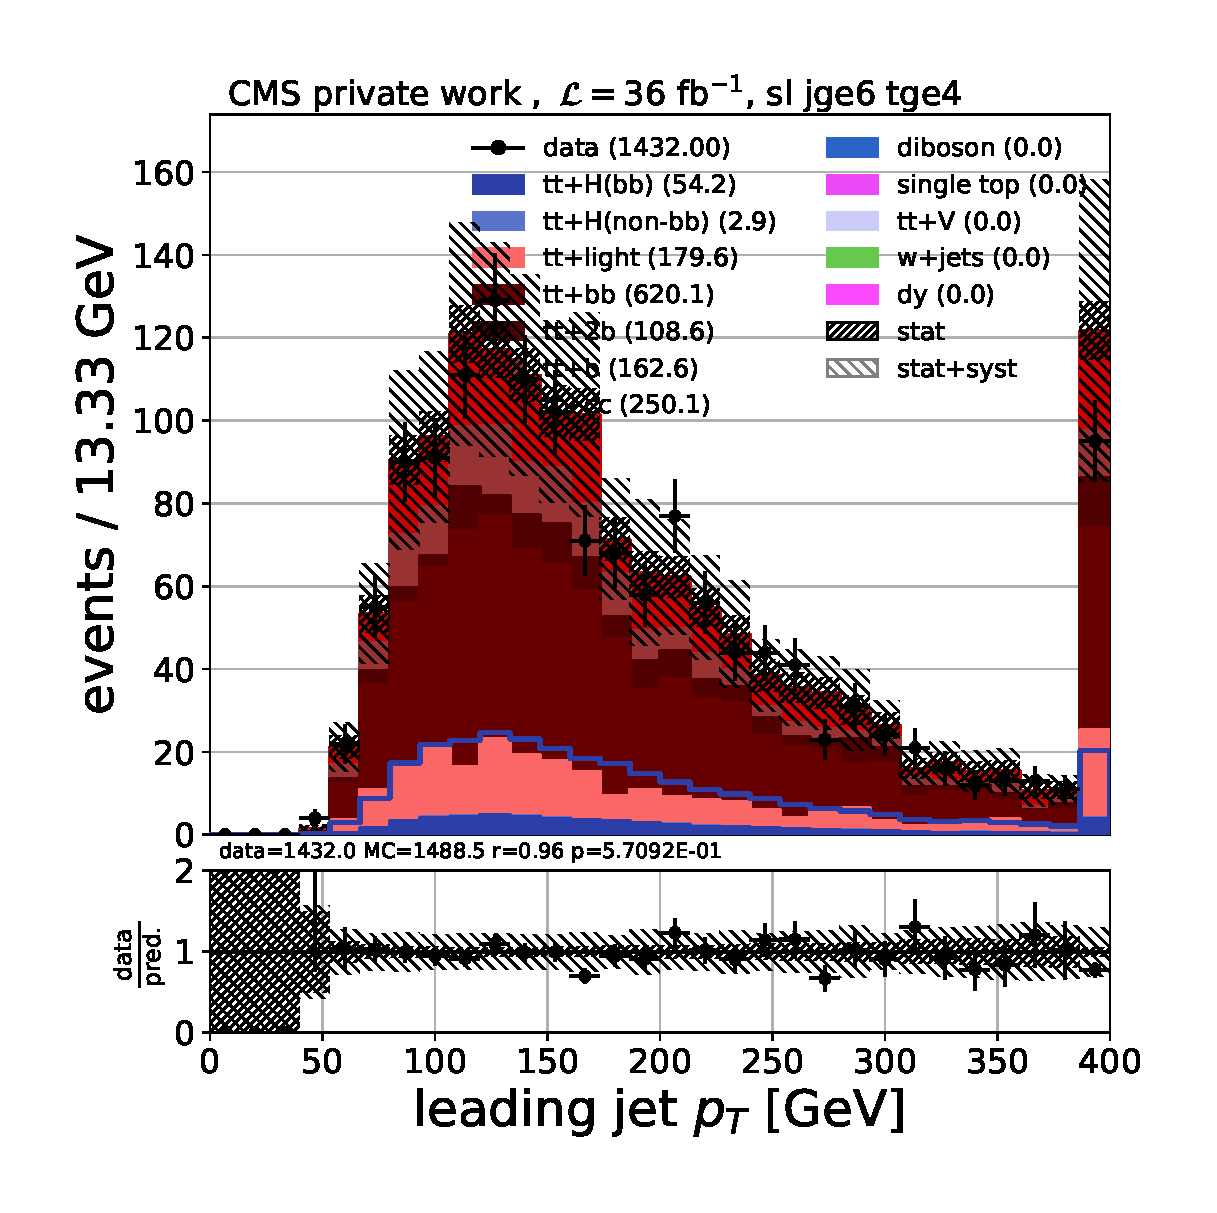
\includegraphics[width=0.4\textwidth]{figures/jetsByPt_0_pt.pdf}} 
\subfloat[fig 2]{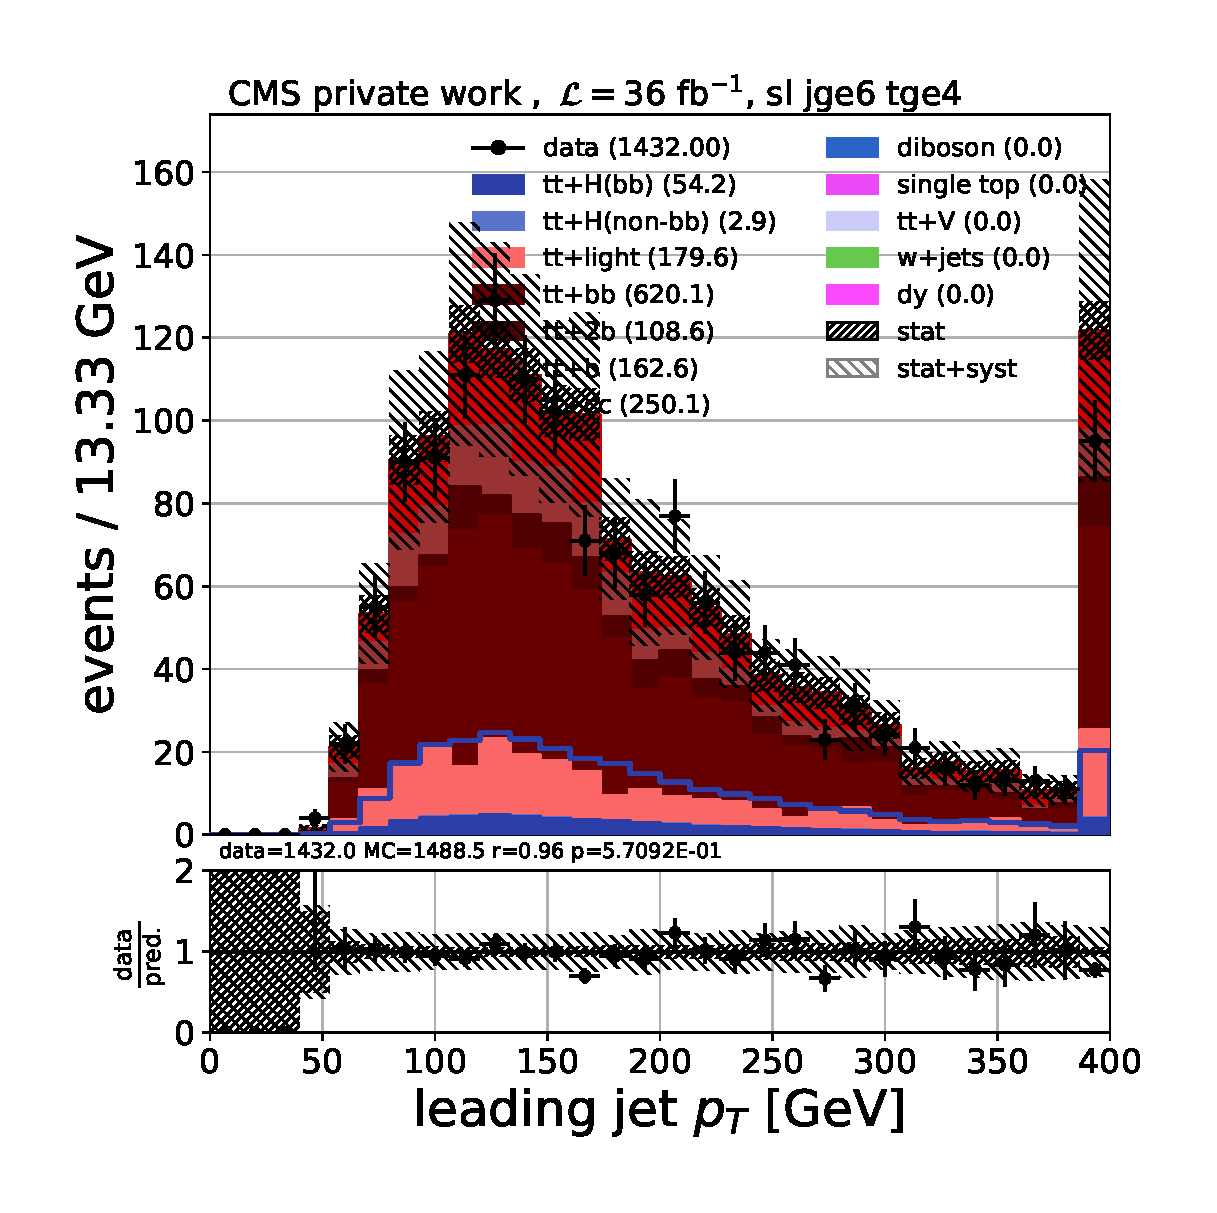
\includegraphics[width=0.4\textwidth]{figures/jetsByPt_0_pt.pdf}}\\
\caption{MEM assumptions.}
\label{fig:mem_assumptions}
\end{centering}
\end{figure}


\subsubsection{Integration}
\label{sec:mem_integration}

The MEM is implemented as a dedicated code in C++, relying on the \texttt{OpenLoops} C++ interface for the evaluation of the hard scattering amplitude. \texttt{ROOT} is used for numerical Lorentz algebra and \texttt{CLING} for interfacing the code to Python. The PDFs are evaluated using the \texttt{cteq66} set via the \texttt{LHAPDF} package. The numerical integration routines rely on the \texttt{VEGAS} algorithm that uses multiple passes to refine the integration grid, with the maximal number of evaluations tuned for approximately $<2.5 \dots 5\%$ numerical accuracy on the integral, suitable for use in a discriminator. We use the \texttt{CUBA} package for numerical integration, as it supports vector-valued integrands. The distribution of expected numerical accuracy is shown on \cref{fig:mem_numerical_accuracy} and illustrates the convergence of the numerical integration. Transfer functions can be provided in a flexible parametrisation using \texttt{ROOT}, however, as described in \cref{sec:mem_optimization}, we have also provided faster, optimized versions of the chosen Gaussian transfer functions. 

\fix Describe integration boundaries.

\begin{figure}
\begin{centering}
\subfloat[fig 1]{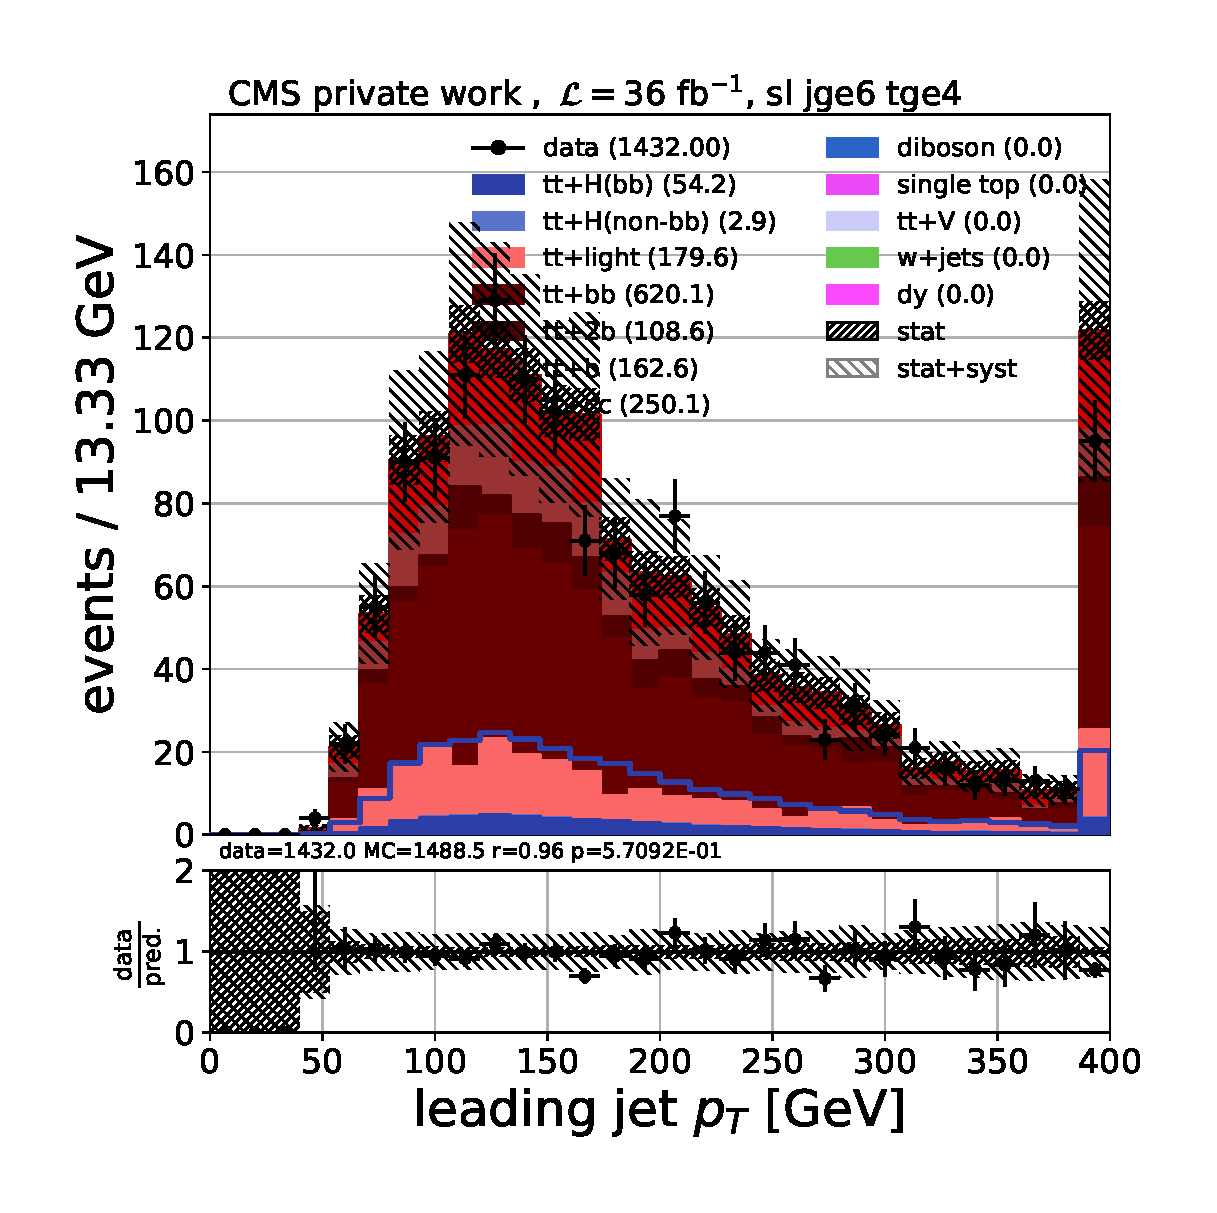
\includegraphics[width = 0.4\linewidth]{figures/jetsByPt_0_pt.pdf}} 
\subfloat[fig 2]{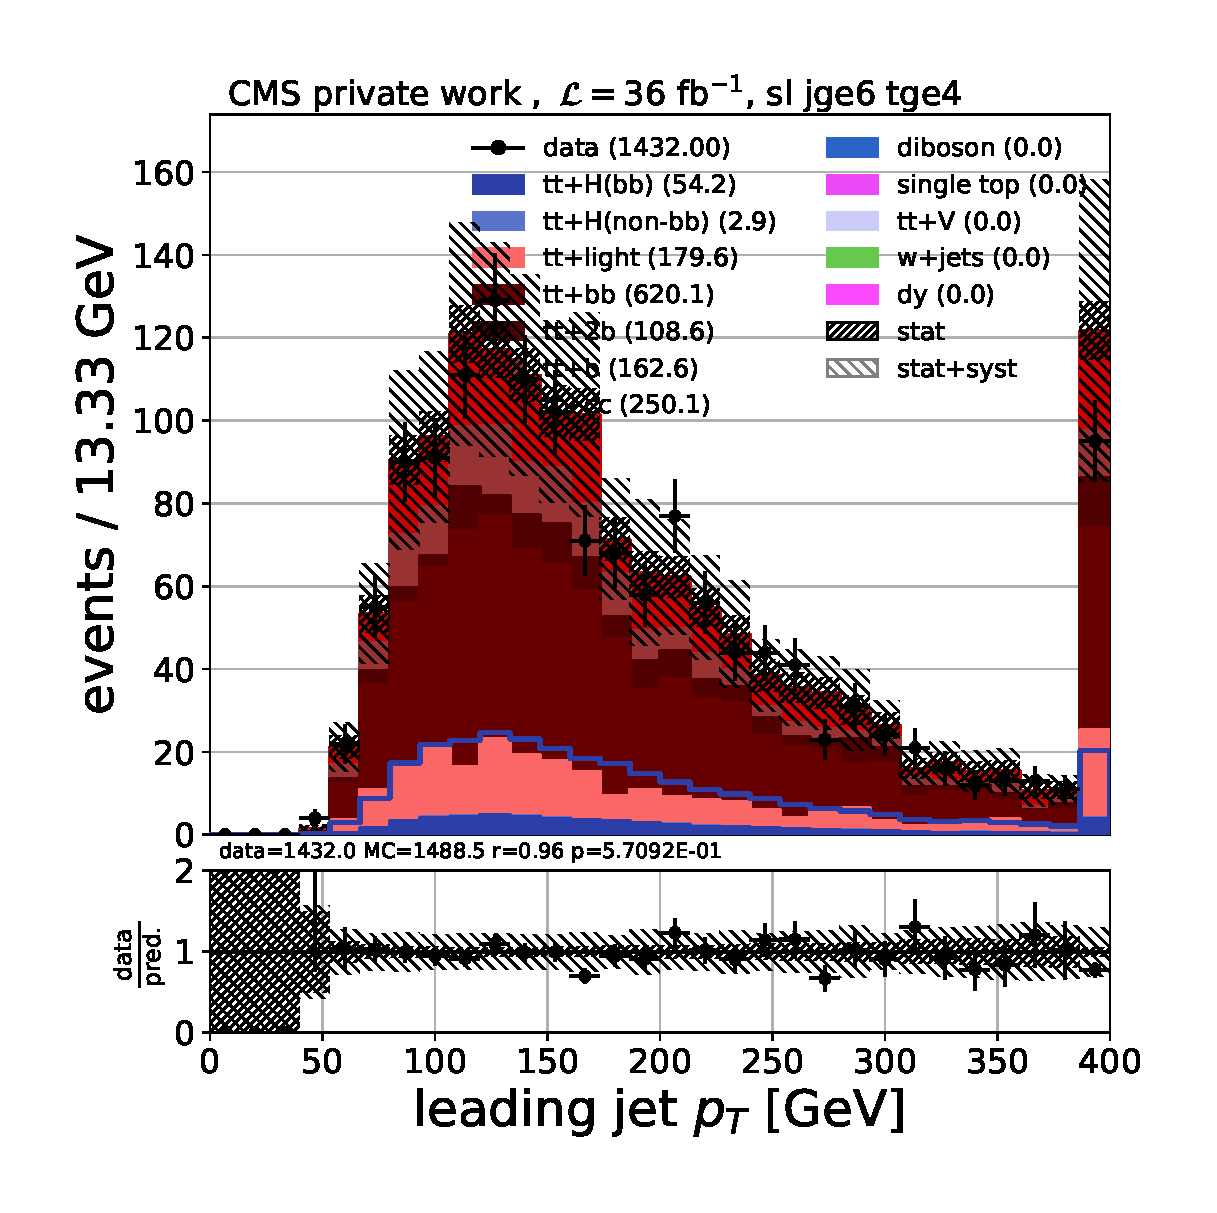
\includegraphics[width = 0.4\linewidth]{figures/jetsByPt_0_pt.pdf}}\\
\caption{MEM assumptions.}
\label{fig:mem_numerical_accuracy}
\end{centering}
\end{figure}

\subsubsection{Profiling and optimisation}
\label{sec:mem_optimization}

In order to optimize the MEM code, we have used the \texttt{igprof} sampling profiler tool to analyze the computational budget spent in various subroutines of the code. In general, we find    
that the overwhelming majority of time is spent within the integrand, out of which about 40\% is spent computing the transfer functions, 35\% is spent evaluating the scattering amplitude of the hard process, 10\% of computing the PDFs and about 10\% on manipulating the phase space volume. The evaluation of the transfer functions at a single phase space point is about an order of magnitude faster than the scattering amplitude. In order to achieve this ratio, we implemented the transfer functions explicitly as optimized C++ functions, instead of relying on a more generic approach using symbolic functions supported in ROOT. Additionally, as we have seen that a large part of time optimising the integration grid is spent in the exponential tails of the transfer function, we have used a piecewise exponential function that is suppressed far in the tails.

Currently, the MEM algorithm as implemented here can only be run on standard x86 CPU architectures. Although it has been shown that GPUs may offer strong parallelization benefits in evaluating the integral, it would be necessary to completely port and optimize the \texttt{OpenLoops} toolset on the GPU in a significant engineering effort\cite{Schouten:2014yza}, furthermore, GPU clusters are currently not commonplace in the WLCG.

\subsubsection{Computational budget}
\label{sec:mem_computational}
In this section, we present a feasibility estimation on using the MEM in a Run II analysis. This is necessary in order to predict the amount of computing resources that will be required. The computing time depends strongly on the number of permutations and integration variables needed for a given interpretation and event topology, as well as the total number of MC simulated events that are needed for the analysis.

\begin{table}[h!]
\begin{center}
\caption{The CPU budget of the MEM. \fix}
\label{tab:mem_cpu_budget}
\begin{tabular}{ccccc}
\hline
category & interpretation & average time & events & total \\
\hline
$1\ell6\mathrm{j}4\mathrm{t}$ & $2_{\mathrm{W}} 2_{\mathrm{h}} 2_{\mathrm{t}}$ & 60 CPUs/ev & 12044 ev & 100 CPUh \\
$1\ell7\mathrm{j}4\mathrm{t}$ & $2_{\mathrm{W}} 2_{\mathrm{h}} 2_{\mathrm{t}}$ & 60 CPUs/ev & 12044 ev & 100 CPUh \\
$1\ell\ge8\mathrm{j}4\mathrm{t}$ & $2_{\mathrm{W}} 2_{\mathrm{h}} 2_{\mathrm{t}}$ & 60 CPUs/ev & 12044 ev & 100 CPUh \\
$1\ell\ge5\mathrm{j}4\mathrm{t}$ & $1_{\mathrm{W}} 2_{\mathrm{h}} 2_{\mathrm{t}}$ & 60 CPUs/ev & 12044 ev & 100 CPUh \\
$1\ell\ge4\mathrm{j}4\mathrm{t}$ & $0_{\mathrm{W}} 2_{\mathrm{h}} 2_{\mathrm{t}}$ & 60 CPUs/ev & 12044 ev & 100 CPUh \\

\hline
\hline
\end{tabular}
\end{center}
\end{table}

\subsubsection{Uncertainties}
\label{sec:mem_uncertainties}

When using the MEM in a realistic experimental analysis, we need to evaluate the effect of systematic uncertainties on the MEM. In general, uncertainties modify the observables $\vec{y} \rightarrow \vec{y}^*$, for example the jet energies may be modified by uncertainties in the jet energy scale calibration. The naive approach to estimate the sensitivity of the discriminator would be to recompute the MEM discriminator weights $P(\vec{y}) \rightarrow P(\vec{y}^*)$. However, this turns out to be impractical, since the number of individual variations that need to be considered can easily reach $\mathcal{O}(10^2)$ and it is not realistic or practical to expend two orders of magnitude more computational resources.
In order to improve the situation, we first note that the variations are generally small, such that $\vec{y}^* \simeq \vec{y} + \delta \vec{y}$. Therefore, the numerical integration described in section \cref{sec:mem_implementation} would be performed on almost the same phase space, with a very similar integration grid.

Furthermore, we see from \cref{eq:definition} that the observables enter the definition of the MEM probability primarily through the transfer functions $W(\vec{y} | \vec{p})$ and affect the integration volume only secondarily. The most computationally costly part in the integrand is the evaluation of the LO scattering amplitudes for the hard process. Therefore, if we can promote the integrand to a vector-valued quantity, such that
\begin{equation}
|\mathcal{M}(\vec{p})|^2 W(\vec{y} | \vec{p}) \rightarrow |\mathcal{M}(\vec{p})|^2  \begin{pmatrix}
  W(\vec{y} | \vec{p}) \\
  W(\vec{y} + \delta \vec{y}_1 | \vec{p}) \\
  \dots \\
  W(\vec{y} + \delta \vec{y}_n | \vec{p})
 \end{pmatrix},
\end{equation}
the integration of the nominal and variated weight can be performed in a single pass using a a grid optimised for the whole integration. We test this approach by comparing the variation evaluated using vector integration to the full computation. As we wish to estimate the sensitivity of the analysis to this uncertainty, it is sufficient if the approximated variation has the same magnitude and direction as the true variation.

Additional complexity is introduced due to variations in the uncertainties possibly changing the topology of the reconstructed final state, as scaling jet energies down may cause jets to migrate under the experimental threshold $p_{T\mathrm{cut}}$. In order to account for this, in case a particular variation $\vec{y} + \delta \vec{y}_n$ changes the reconstructed final state, the MEM is still recomputed from scratch.

\subsubsection{MEM on the WLCG}

From \cref{sec:mem_computational} it is apparent that it is necessary to compute the MEM on distributed systems in order to have a reasonable turn-around time for the analysis. Therefore, we have parallelized the workflow both on the level of a computing cluster using \texttt{grid-control} and the WLCG using \texttt{CRAB}. On the WLCG, we have thus been able to take advantage of CMS computing resources opportunistically and have demonstrated that the MEM as implemented here is able to run on a wide range of data centers on a planetary scale. For this, we relied on \texttt{CMSSW} to provide a consistent environment along with user-provided external dependencies such as \texttt{OpenLOOPS}. We integrated the MEM into a multi-step workflow that produced the final analysis data sets directly from CMS MiniAOD in a single pass. This way, we were able to benefit from load balancing using data locality in CMS and reduced the number of manual intermediate steps and data management which can be error prone.
% asdasd \ttH

\subsection{Expected performance}
We demonstrate the expected performance of the MEM on a MC simulation sample of \ttH and \ttbar+jets. First, on \cref{fig:mem_proba}, we verify that the signal and background probabilities indeed behave as expected on their respective MC simulations.

\begin{figure}
\begin{centering}
\subfloat[MEM probability for the \ttH hypothesis.]{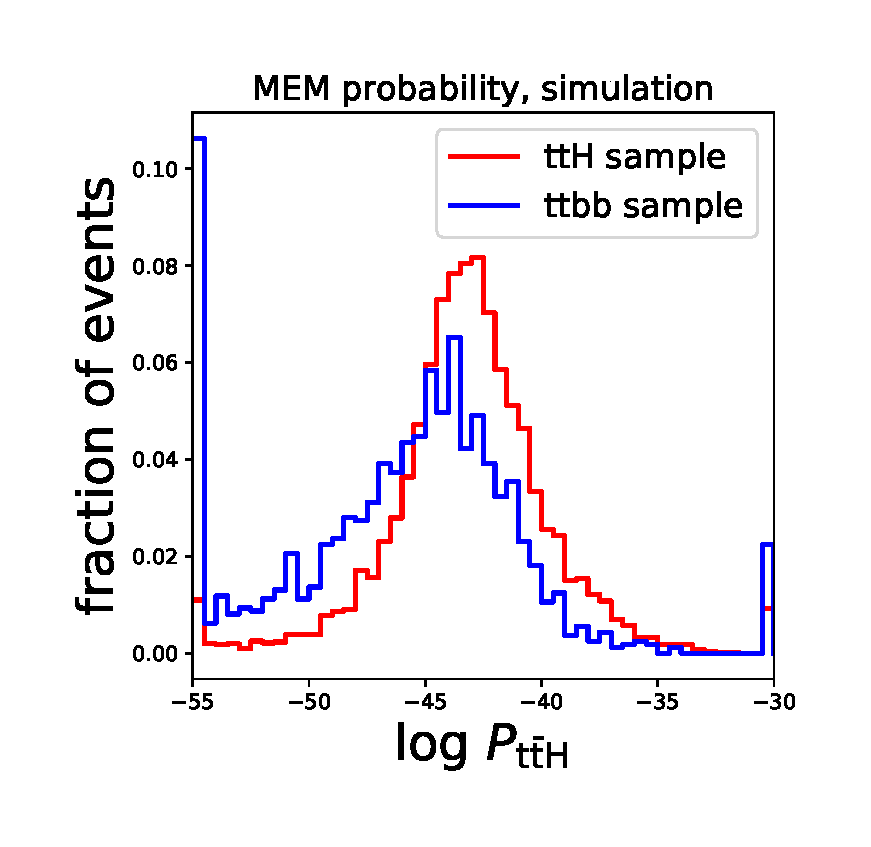
\includegraphics[width = 0.5\textwidth]{figures/mem_proba_tth.pdf}} 
\subfloat[MEM probability for the \ttbb hypothesis]{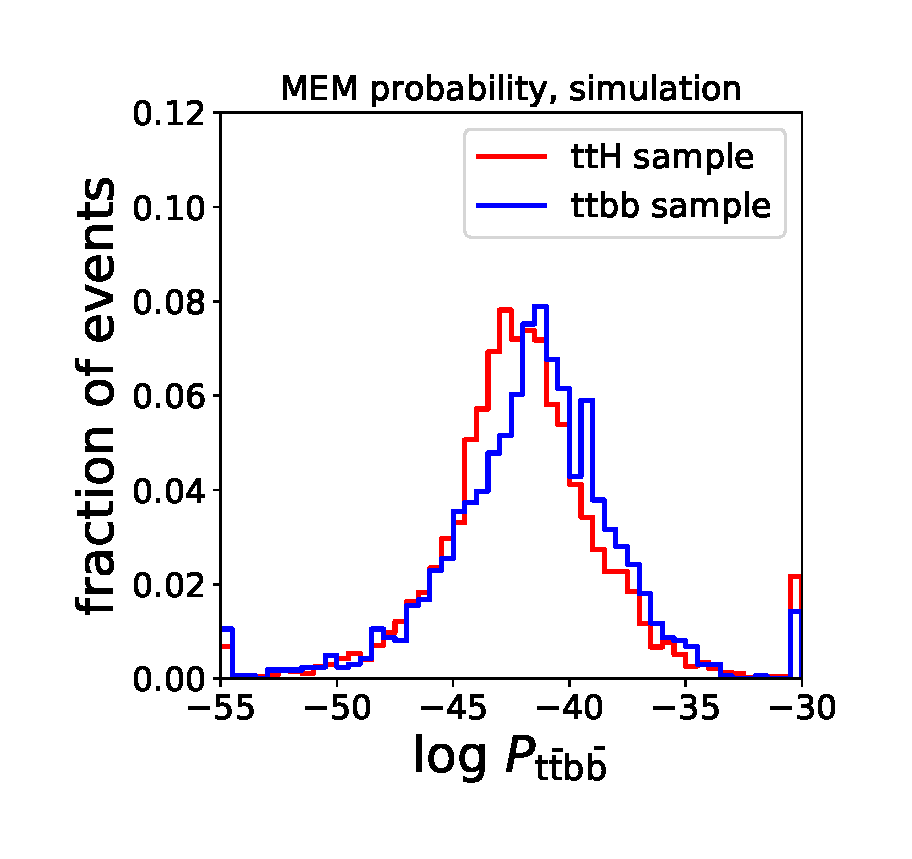
\includegraphics[width = 0.5\textwidth]{figures/mem_proba_ttbb.pdf}}\\
\caption{The expected distribution of the signal probability $P_{\ttHbb}$ and the background probability $P_{\ttbb}$ on MC simulation. We see that for the signal sample, the signal probability is on average higher than the background probability, and vice versa for the background. Here, we have selected events with exactly 1 isolated lepton, at least 6 jets, out of which 4 must be b tagged. Furthermore, the jets are required to be matched to quarks from the corresponding hard interaction on generator level.}
\label{fig:mem_proba}
\end{centering}
\end{figure}

\begin{figure}
\begin{centering}
\subfloat[fig 2]{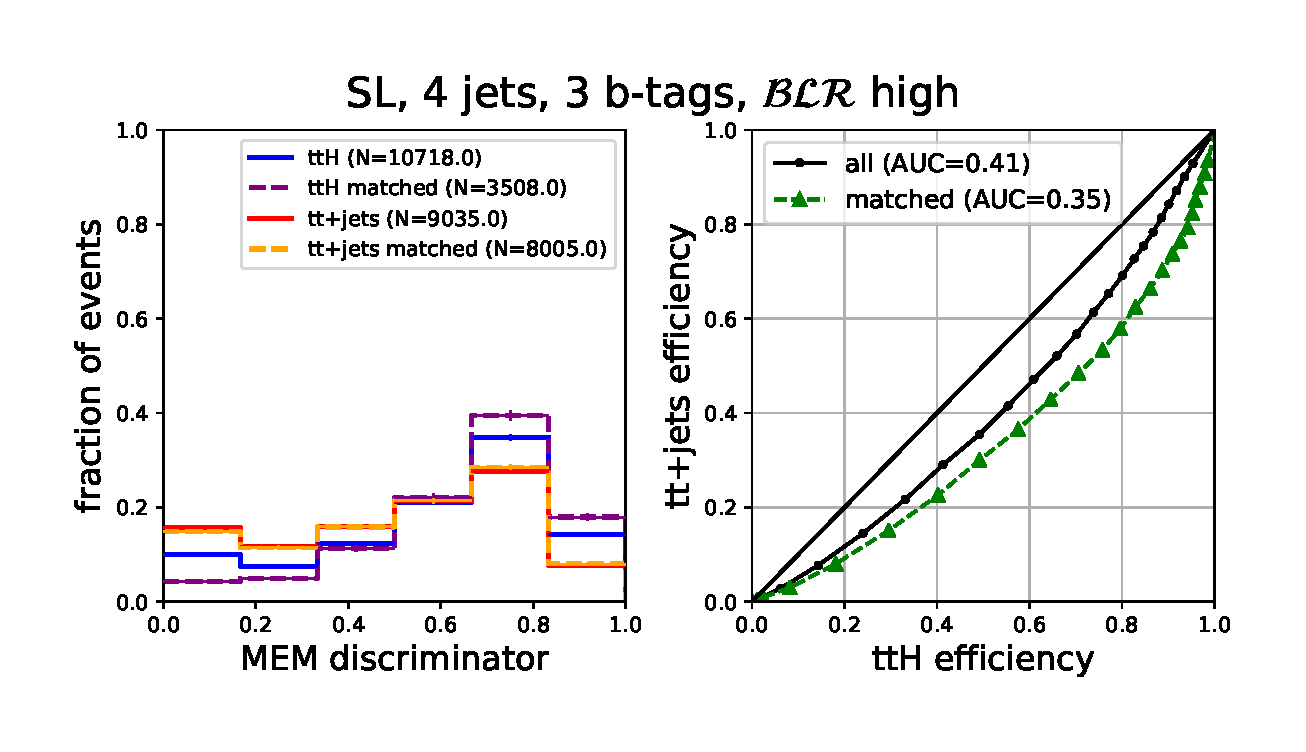
\includegraphics[width = 1.0\textwidth]{figures/mem_sl_j4_t3_blrH.pdf}}\\
\subfloat[fig 1]{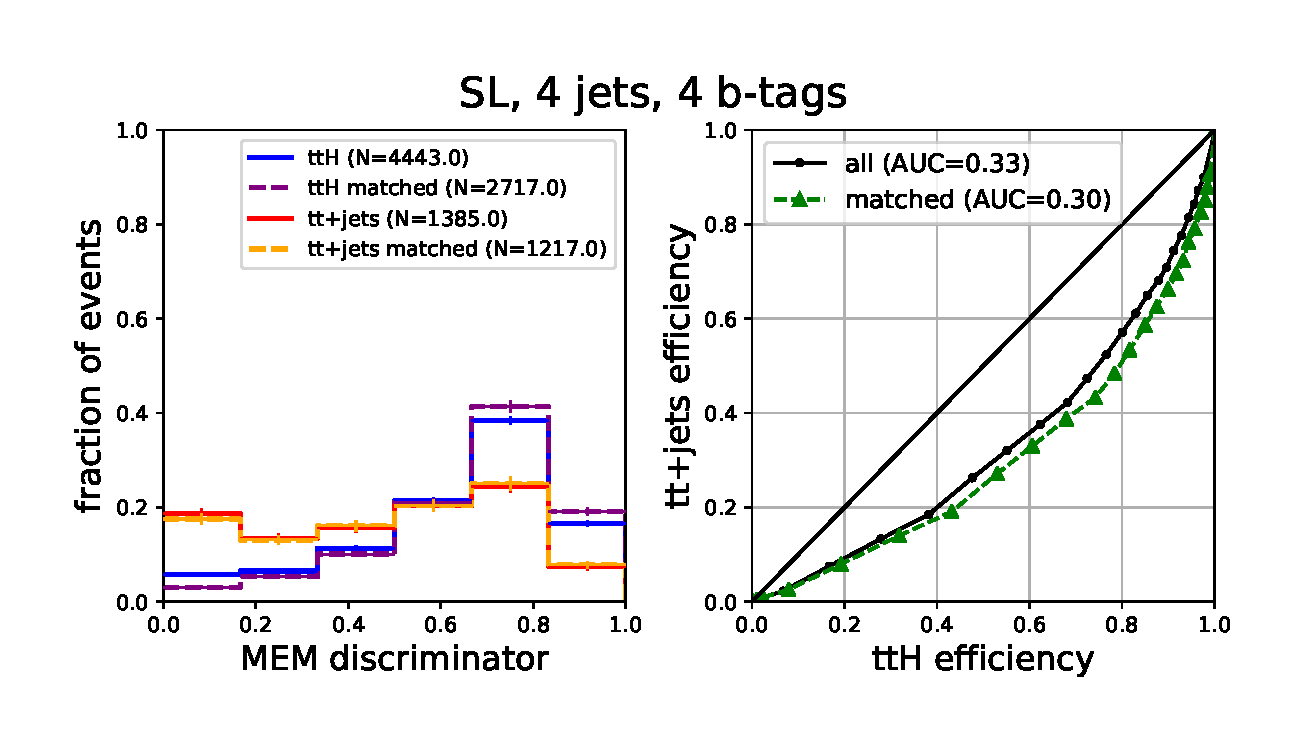
\includegraphics[width = 1.0\textwidth]{figures/mem_sl_j4_t4.pdf}}\\
\caption{Add your own figures before compiling}
\label{fig:some_example}
\end{centering}
\end{figure}

\begin{figure}
\begin{centering}
\subfloat[fig 2]{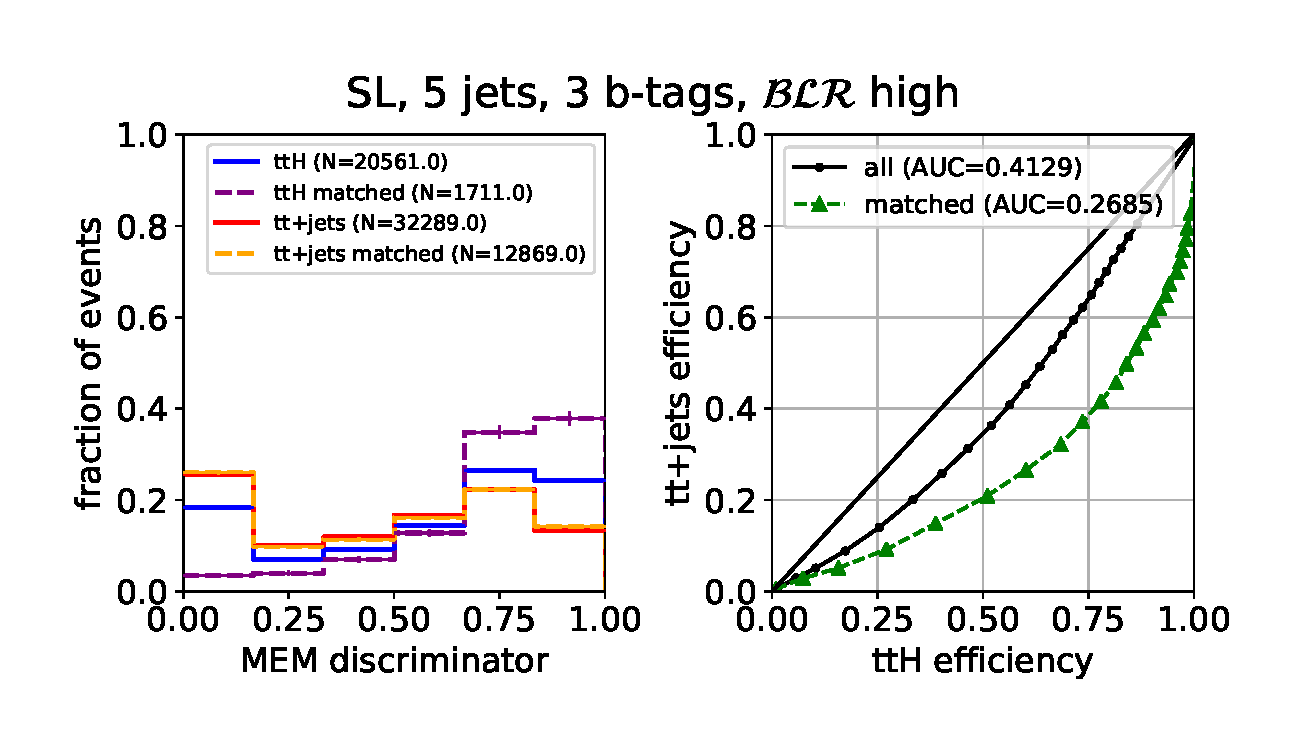
\includegraphics[width = 1.0\textwidth]{figures/mem_sl_j5_t3_blrH.pdf}}\\
\subfloat[fig 1]{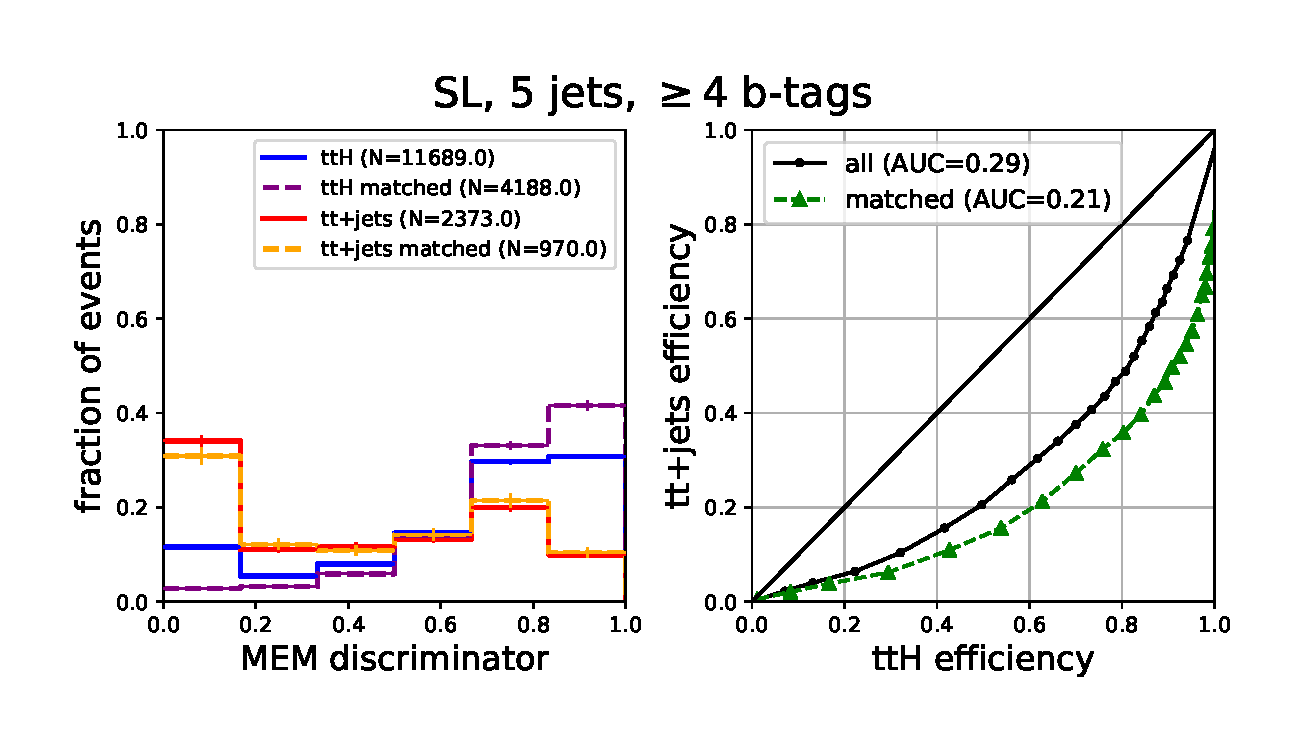
\includegraphics[width = 1.0\textwidth]{figures/mem_sl_j5_tge4.pdf}}\\
\caption{Add your own figures before compiling}
\label{fig:some_example}
\end{centering}
\end{figure}

\begin{figure}
\begin{centering}
\subfloat[fig 1]{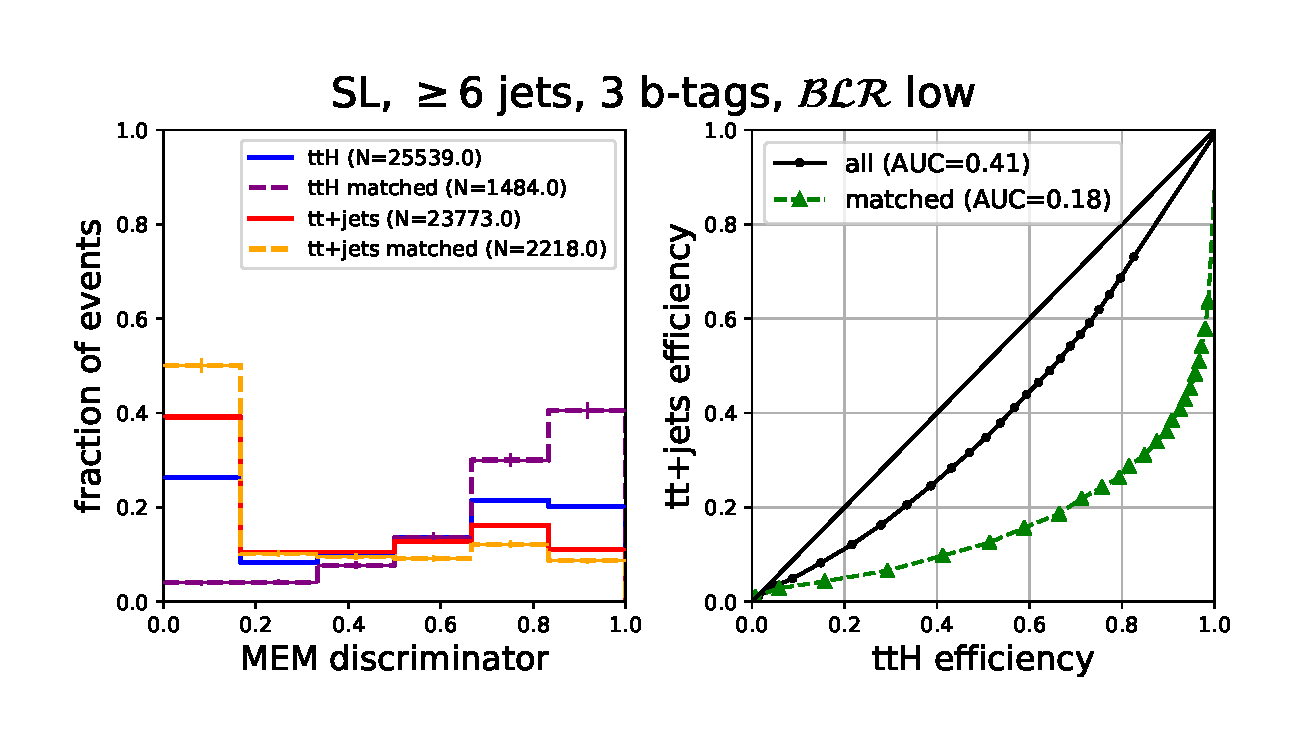
\includegraphics[width = 1.0\textwidth]{figures/mem_sl_jge6_t3_blrL.pdf}}\\
\subfloat[fig 2]{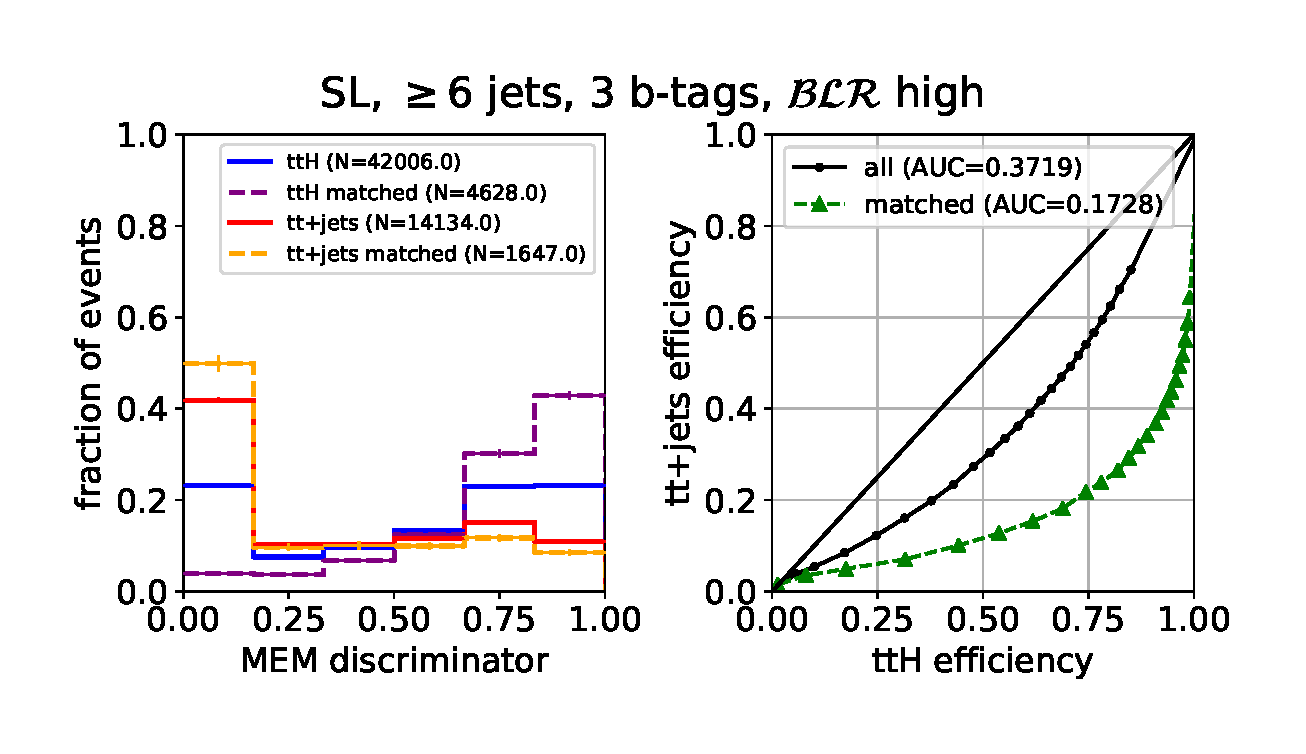
\includegraphics[width = 1.0\textwidth]{figures/mem_sl_jge6_t3_blrH.pdf}}\\
\caption{Add your own figures before compiling}
\label{fig:some_example}
\end{centering}
\end{figure}

\begin{figure}
\begin{centering}
\subfloat[fig 3]{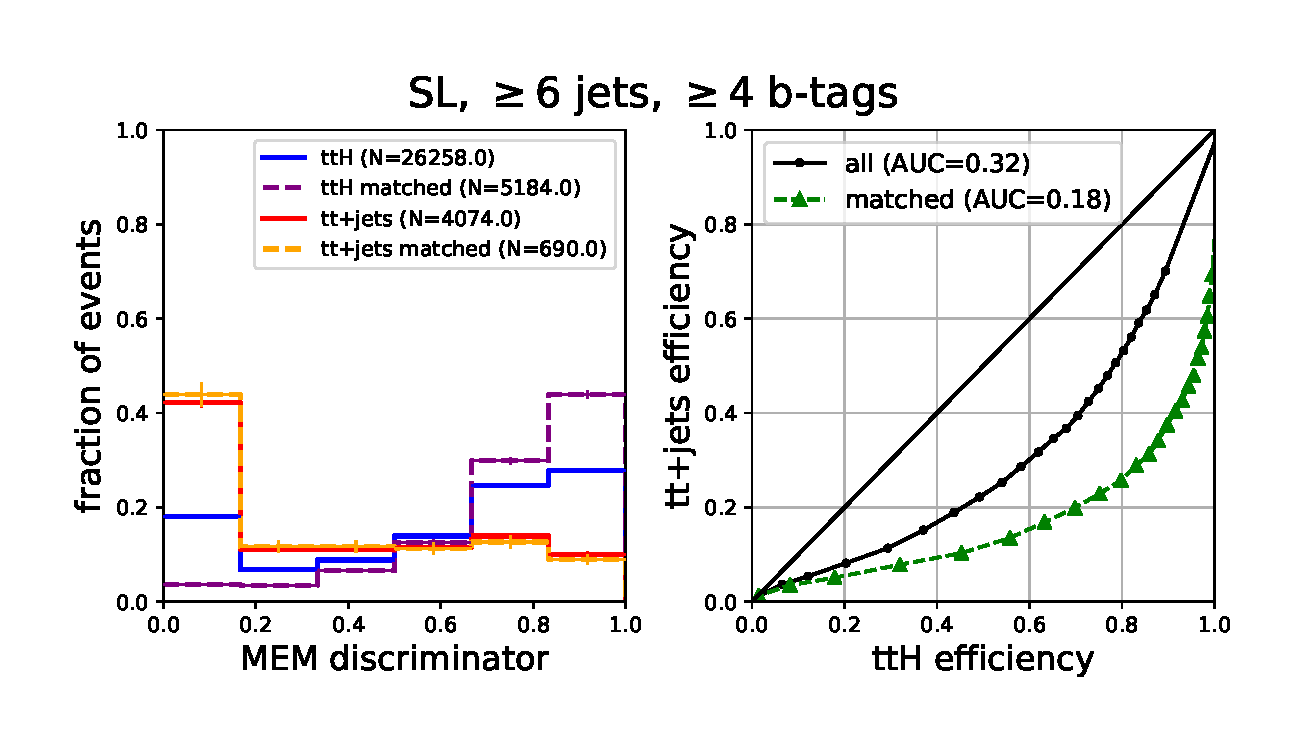
\includegraphics[width = 1.0\textwidth]{figures/mem_sl_jge6_tge4.pdf}}\\
\subfloat[fig 4]{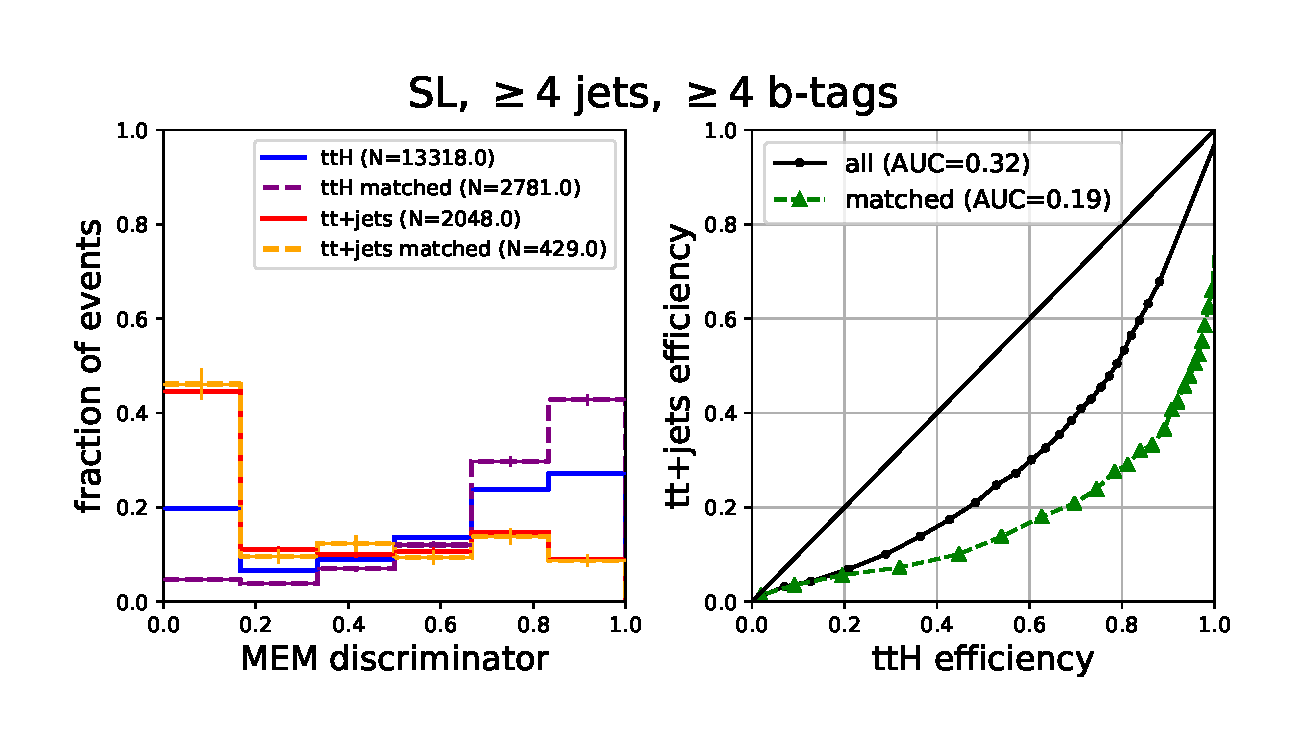
\includegraphics[width = 1.0\textwidth]{figures/mem_sl_jge7_tge4_7jet.pdf}}\\ 
\caption{Add your own figures before compiling}
\label{fig:some_example}
\end{centering}
\end{figure}


% \begin{figure}
% \begin{centering}
% \subfloat[fig 1]{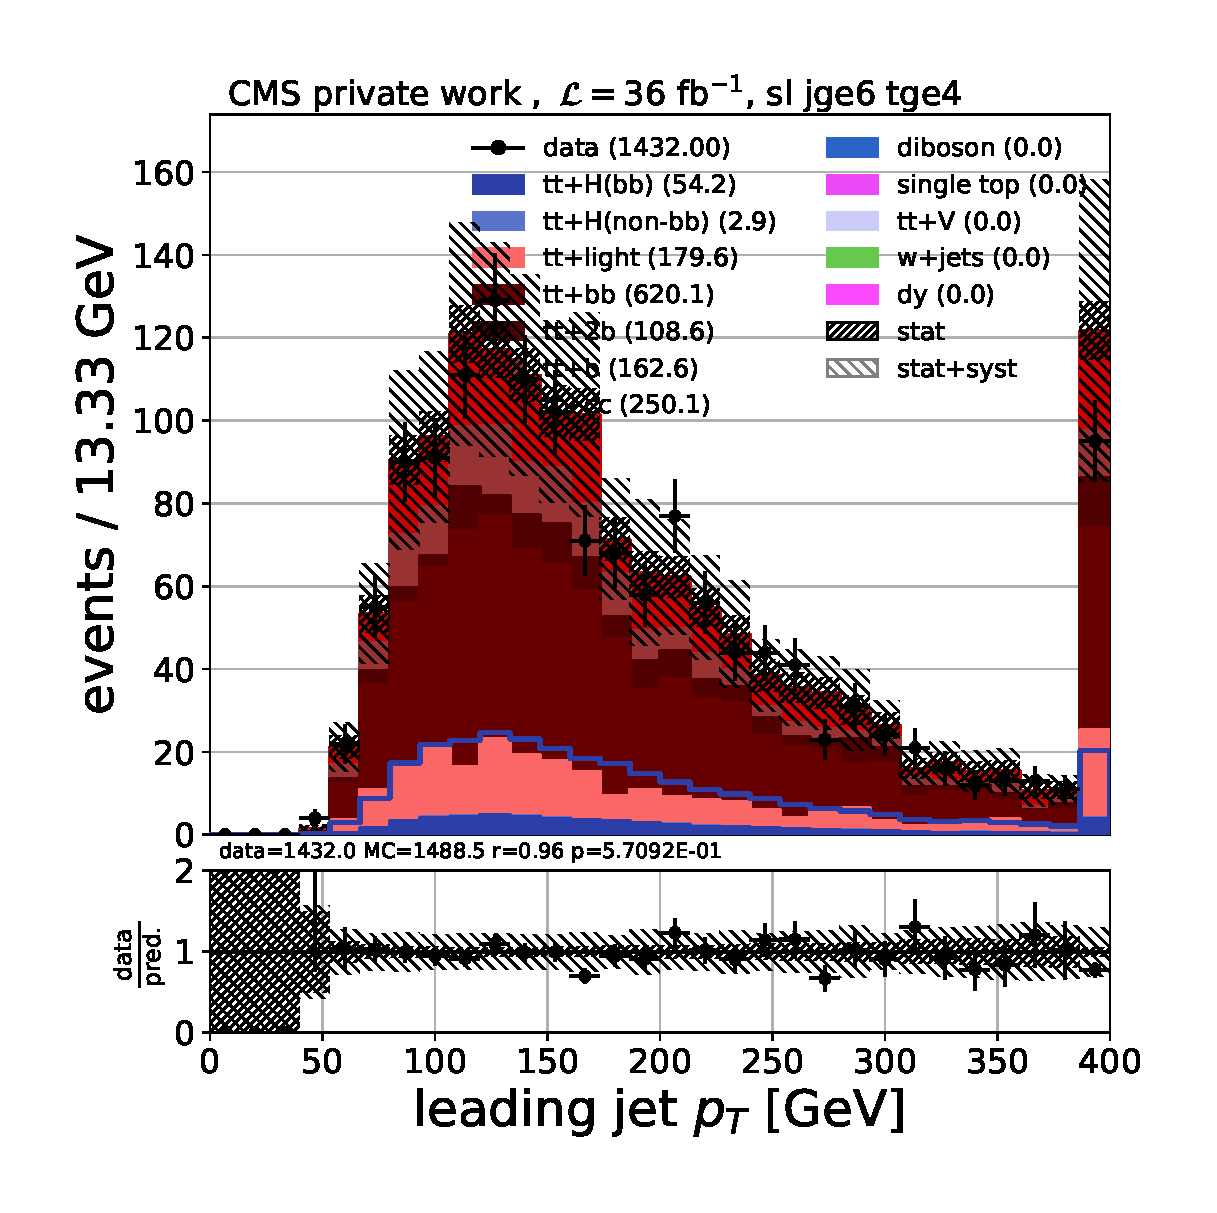
\includegraphics[width = 0.4\linewidth]{figures/jetsByPt_0_pt.pdf}} 
% \subfloat[fig 2]{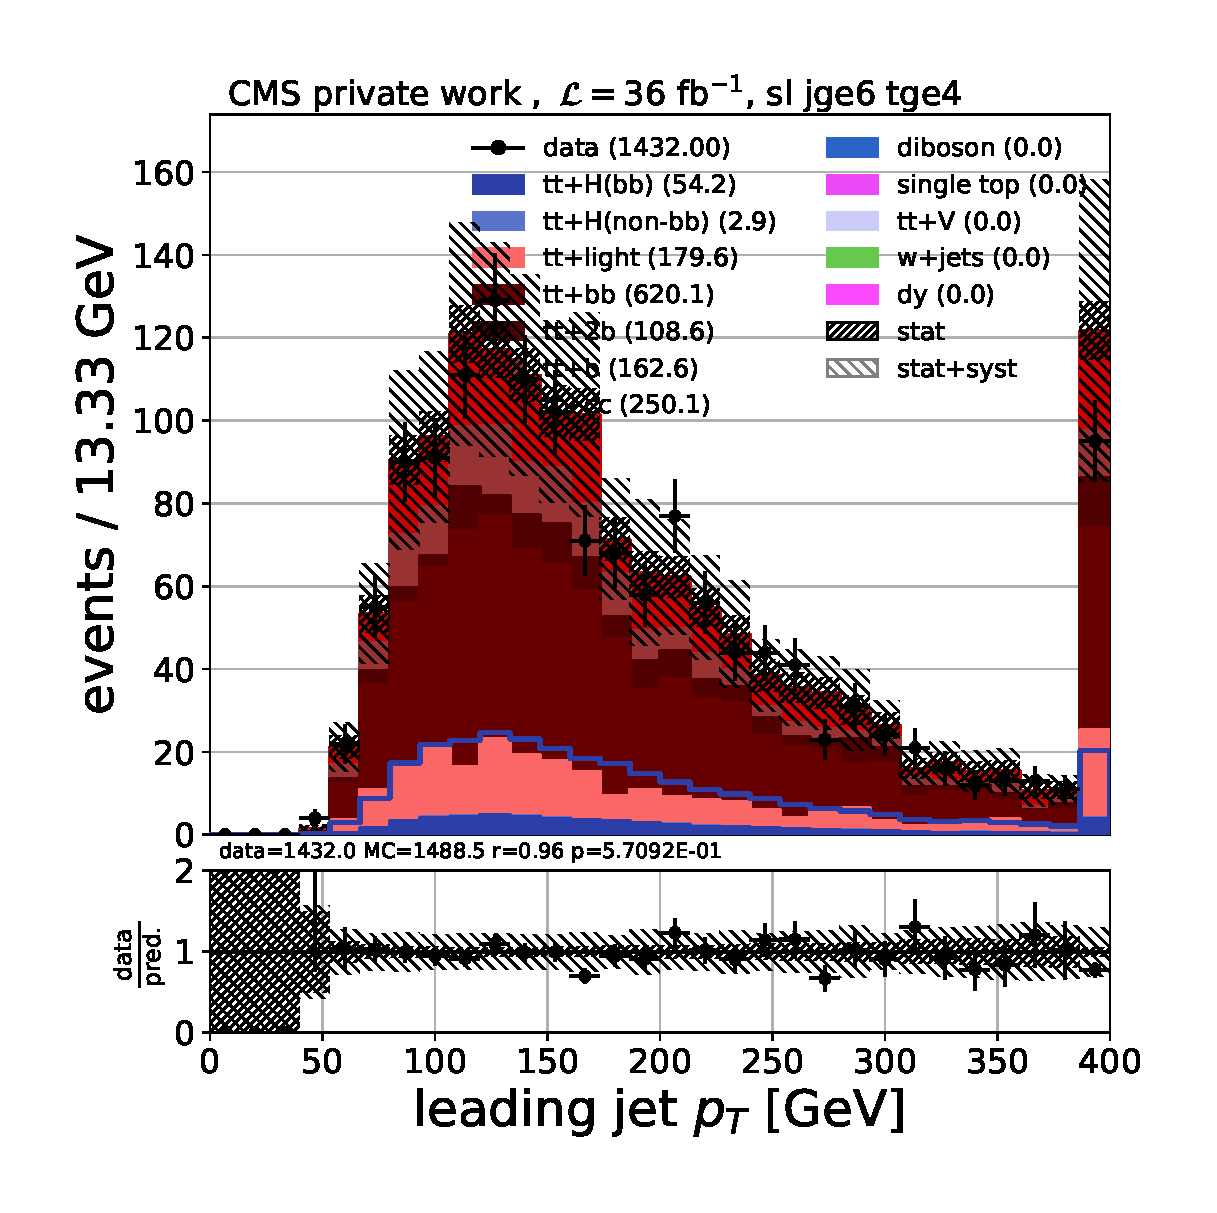
\includegraphics[width = 0.4\linewidth]{figures/jetsByPt_0_pt.pdf}}\\
% \subfloat[fig 3]{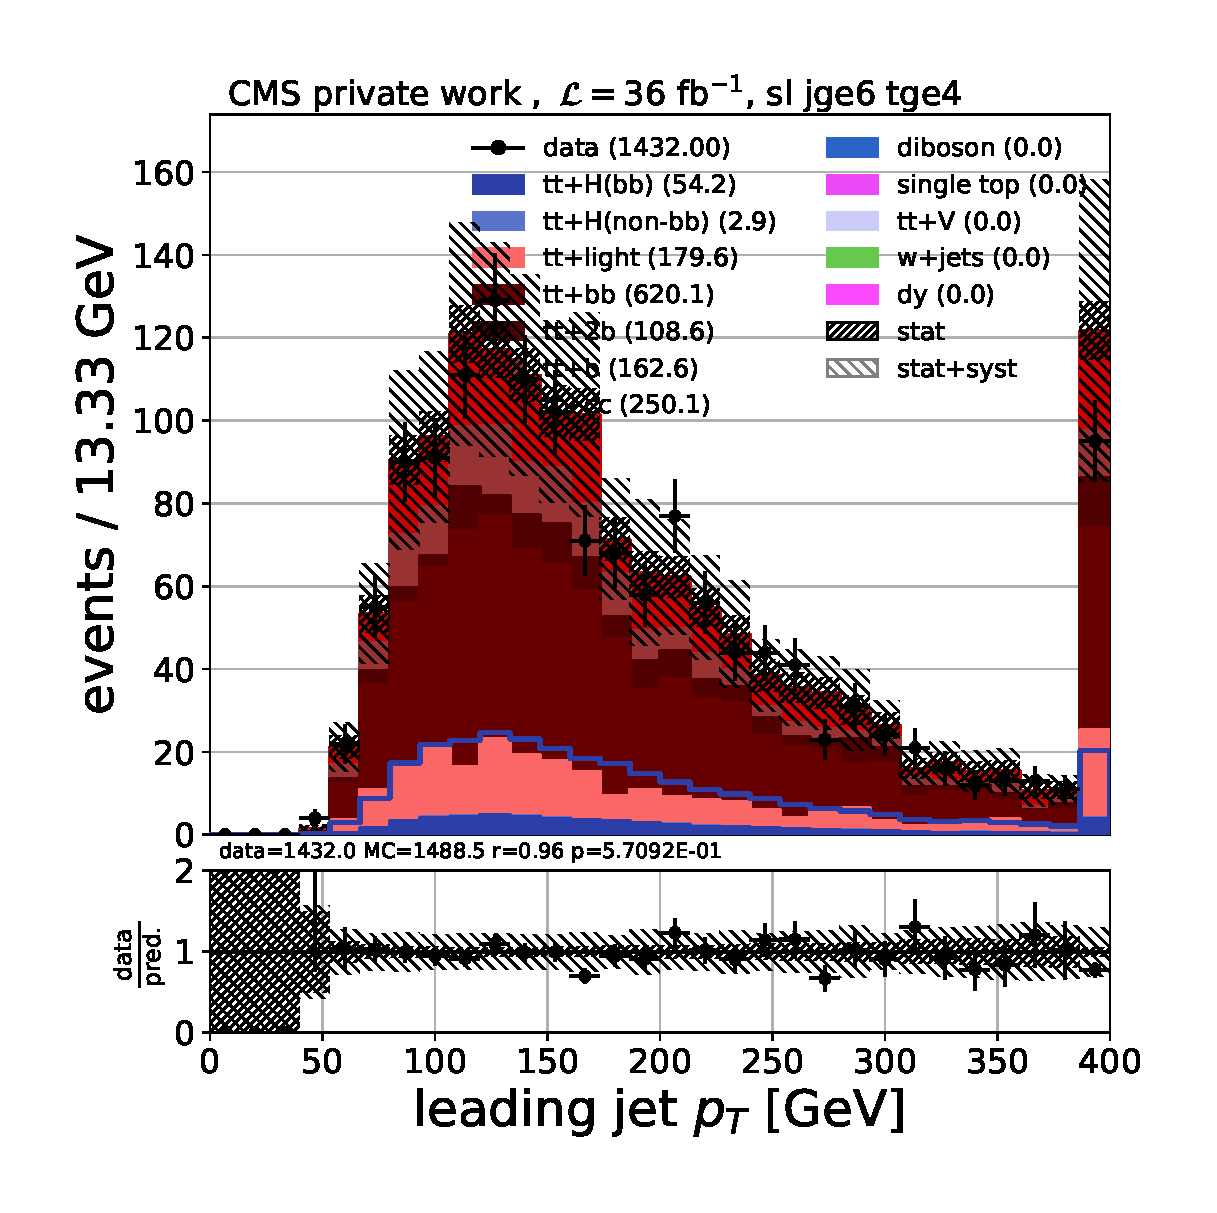
\includegraphics[width = 0.4\linewidth]{figures/jetsByPt_0_pt.pdf}}
% \subfloat[fig 4]{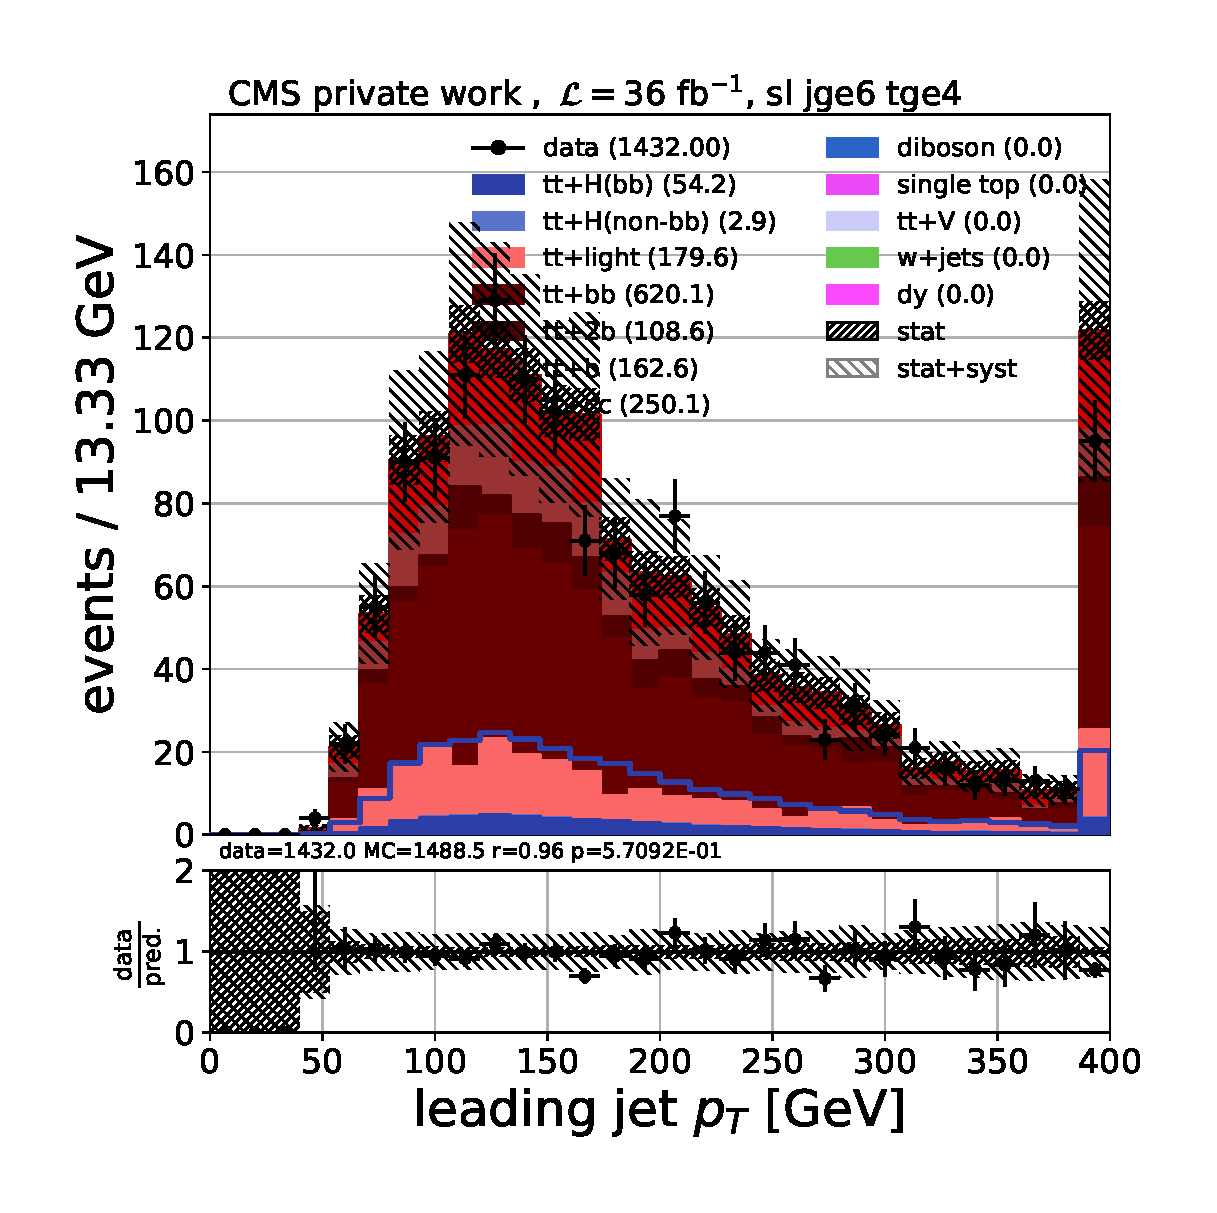
\includegraphics[width = 0.4\linewidth]{figures/jetsByPt_0_pt.pdf}} 
% \caption{Add your own figures before compiling}
% \label{fig:some_example}
% \end{centering}
% \end{figure}

% On \cref{fig:some_example} bla bla
\section{Search for \ttHbb}

In this chapter, we will describe the search for \ttHbb using the MEM at the CMS experiment. This is based on preliminary results from CMS\cite{CMS-PAS-HIG-16-038} and ongoing work. We concentrate on the SL and DL decay channels of the top pair and the application of the MEM in the search for \ttHbb, where various subprocesses of \ttbar+jets are the primary irreducible background. Whenever we show results using CMS data, we use those plots and data that have been publicly released by the CMS collaboration.

Briefly, the analysis proceeds as follows. First, we select events with at least 1 (2) charged lepton(s) in the SL (DL) top decay channels and at least 4 jets, out of which 3 must be b tagged. The detailed identification criteria for the physics objects (jets and leptons) are motivated by established top quark analyses and are described in \cref{sec:object_id}. We then further divide the events into independent categories based on the jet and b tag multiplicity, described in \cref{sec:categories}. This is done in order to constrain the various subprocesses of \ttbar, described further in \cref{sec:ttbar_subprocesses}. In order to extract the signal strength $\mu$, we perform a combined template fit across all the categories, relying on the discriminating power provided by the MEM in categories with a high signal-to-background ratio and on other multivariate techniques in background-enhanced (control) regions. The fit is described in \cref{sec:statistical_method}.
A crucial component in the fit is the estimated systematic uncertainty, which drives the determination of the confidence interval of the estimated signal strength and is described in \cref{sec:systematics}. Throughout, we use MC simulation and data samples described in \cref{sec:data_mc}.

\subsection{Data and simulation}
\label{sec:data_mc}

We use proton-proton collision data collected by the CMS experiment at a center-of-mass energy of $\sqrt{s} = 13~\mathrm{TeV}$, corresponding to a total integrated luminosity of $12.9~\ifb$ in the SL channel and $11.4-12.9$ in the DL channel, denoted the CMS ICHEP2016 data set. The smaller amount of integrated luminosity for the DL channel is due to disabled $\mathrm{e}^+\mathrm{e}^-$ trigger paths disabled during data taking. We are currently working on publishing results with the full 2016 dataset of about $36~\ifb$, however, we cannot show the data before it is made public by the Collaboration.

We use MC generators to model the signal and background processes, interfaced to a parton shower and hadronization where appropriate. In order to model the detector effects, we use a detailed simulation of the reconstruction, selection efficiencies and detector resolutions based on \geant.

For the \ttH signal, \ttbar and single-top backgrounds, we use the NLO generator \powheg (v.2)\cite{Frixione2007,Re2011}. The use of an NLO model for the signal and main background modelling is a significant advancement over Run I analyses, where only a LO model was available. Besides \ttbar, we need to model the production of W or Z/$\gamma^*$ bosons with additional jets (denoted W/Z+jets or commonly V+jets), which are simulated using MADGRAPHATNLO (v. 2.2.2) and diboson production (WW, WZ, ZZ), simulated using \pythia (v. 8.2).

Throughout, we assume the value of the top quark mass to be $172.5\GeV/c^2$ and of the Higgs boson to be $125\GeV/c^2$. In order to describe the substructure of the protons via the parton density functions, we use the PDF parametrization provided by NNPDF3.0 and \pythia for showering and hadronization.

In order to model the production of hadrons, the parameters in the \pythia model have been tuned to historical Tevatron, LEP and LHC data\cite{CMS-PAS-GEN-14-001,Skands:2014pea}. In moving to $\sqrt{s} = 13~\TeV$, we have found that the default tune in \pythia does not reproduce the observed number of jets in data. Therefore, CMS has created a custom tune where the $\alpha_{\mathrm{ISR}}$, which controls the amount of initial-state radiation, and $h_{\mathrm{damp}}$, which suppresses real emissions in \powheg, have been adapted to reproduce the spectrum of the number of jets observed at CMS\cite{CMS-PAS-TOP-16-021}. This has been done on $\sqrt{s} = 8~\TeV$ data and significantly improves the modelling of the jet multiplicity.

We list the details of the MC samples in \cref{tab:mc_samples} and of data in \cref{tab:data_samples}.

\begin{table}[h!]
\begin{center}
\caption{The MC samples.}
\label{tab:mc_samples}
\begin{tabular}{cccc}
\hline
sample & generator & events & cross-section \\
\hline
\ttHbb & \powheg (NLO) and \pythia & 100k & 123 pb \\
\ttHnonbb & \powheg (NLO) and \pythia & 100k & 123 pb \\
\ttbar & \powheg (NLO) and \pythia & 100k & 123 pb \\
\hline
\hline
\end{tabular}
\end{center}
\end{table}

\begin{table}[h!]
\begin{center}
\caption{The data samples.}
\label{tab:data_samples}
\begin{tabular}{cccc}
\hline
trigger & run period & integrated luminosity \\
\hline
SingleMuon & Run B & $12.9~\ifb$ \\
\hline
\hline
\end{tabular}
\end{center}
\end{table}

In order to compare simulation to data, the simulated events are weighted according to the integrated luminosity and the predicted cross sections, which are taken from inclusive calculations. In particular, the \ttH cross section is known at NLO accuracy\cite{Dittmaier:1318996,Beenakker:2001rj,Beenakker:2002nc,Dawson:2002tg,Dawson:2003zu}. The Higgs boson branching fraction for \Hbb is affected by radiative corrections that are known up to N4LO (QCD) and NLO (EWK), resulting in an uncertainty of about 1-2\% \cite{Djouadi:1997yw,Butterworth:2010ym,deFlorian:2016spz}.
The cross section for \ttbar is know at NNLO accuracy and includes soft gluon resummation to NNLL\cite{Czakon:2011xx}. The cross-sections of the minor backgrounds are known to at least NLO, as summarized in \cref{tab:mc_samples}.

In addition to the hard interaction and the consequent showering and hadronization, events from additional pp interactions within the same bunch crossing are superimposed on the simulated event for all processes. The multiplicity distribution of these additional pileup events is reweighted to match the observed number of interactions in data. Furthermore, we correct the MC simulation with additional data-driven correction factors for b tagging, lepton efficiencies, described in \cref{sec:systematic_unc}.

\subsubsection{Modelling of \ttbar}
\label{sec:ttbar_subprocesses}
We subdivide the \ttbar sample further based on the generator-level flavor of additional jets, as the theoretical uncertainties of these subprocesses are uncorrelated and therefore need to be treated separately. In particular, we distinguish between
\begin{itemize}
\item \ttbb, where two additional bottom jets are created from one or more B hadrons,
\item \ttb with only one additional bottom jet,
\item \tttwob where jets from two B hadrons merge to produce one resolved bottom jet,
\item \ttcc if there are no additional bottom jets and at least on charm jet,
\item \ttlf in case there are no bottom or charm jets.
\end{itemize}
Despite considerable advances in theoretical modelling, the theoretical uncertainties in \ttbar + heavy flavour production are still significant\cite{Cascioli:2013era}. The aim of this splitting is to have an experimental way of constraining uncertainties on the various \ttbar~subprocesses.

The jet flavour is assigned using so-called \textit{ghost clustering}, where simple geometrical matching between partons and jets is superceded by clustering the partons and hadrons along with the jet constituents using standard jet algorithms. Furthermore, information from the generator-level decay chain is used assign the flavour of the jet according to the parton that gave rise to that jet\cite{Bartosik:2047049}.

\subsection{Event reconstruction and object identification}
\label{sec:object_id}
We use particle-flow to reconstruct events from particle candidates based on signals from all sub-detectors. This allows us to perform the analysis at the level of physics objects, namely, jets and leptons\cite{cms_particleflow:2017}. In order to mitigate the effects of pileup, we identify the primary vertex associated with the hard interaction by requiring $n_{\mathrm{dof}} > $, $|z| < 24~\mathrm{cm}$ and $|rho|<2~\mathrm{cm}$. The charged hadrons that are associated to pileup vertices are not included in the subsequent event reconstruction \cite{CMS:2014ata}.

Our final state of interest contains charged leptons ($\mathrm{e}^\pm$, $\mathrm{\mu}^\pm$), jets from light quarks and bottom quarks and \MET. This is due to the decay of the top quark, which in the standard model happens almost exclusively through $\mathrm{t} \rightarrow \mathrm{W} \mathrm{b}$.

\subsubsection{Charged leptons}
\label{sec:object_id_lep}

The leptonic decay of at least one of the W-bosons is required in order to pass the trigger selection. In order to suppress leptopns from the multi-jet QCD background, the charged leptons are required to be sufficiently isolated from hadronic activity using an isolation variable, which is computed within a cone of radius $\Delta R$ around the lepton direction (defined by the track) from the primary vertex as shown in \cref{eq:iso_mu} for muons and \cref{eq:iso_el} for electrons. In order to evaluate the isolation, we sum over the transverse momenta of all particle candidates ($p_T^{c.h.}$ for charged hadrons, $E_T^{n.h.}$ for neutral hadrons, $E_T^{\gamma}$ for photons) excluding the lepton itself and subtracting the neutral component from pileup events based on either the average pile-up energy ($\rho$) and effective area ($A$) for electrons or pile-up associated charged hadrons for muons. The prefactor $1/2$ for the pile-up component for muons is used to account for the approximate charged-to-neutral fraction in the hadronization of pile-up interactions\cite{CMS:2012}.

Furthermore, in order to supress leptons from non-prompt decays, we apply identification criteria based on various reconstruction parameters on the leptons. For muons, we apply the tight ID, which is a cut-based selection that suppresses decays in flight and is based on properties of the global track fit, number of hits in the pixel detector, tracker and muon chambers and sufficient proximity to the primary vertex\cite{Chatrchyan:2012xi,CMS:2017_muon_pog}. For electrons, the ID is based on a multivariate discriminator combining track-to-cluster matching observables, supercluster structure and cluster shapes \cite{Khachatryan:2015hwa,CMS:2017_egamma_pog}.

We summarize the lepton selection criteria in all the considered channels in table \cref{tab:lepton_selection} and describe the event selection further in \cref{sec:event_selection}.

\begin{equation}
\label{eq:iso_mu}
\mathrm{Iso}_{\mathrm{\mu}} = \sum_{\Delta R < 0.4} p_T^{c.h.} + \mathrm{max}\biggl(0, \sum_{\Delta R < 0.4} [E_T^{n.h.} + E_T^{\gamma} - \frac{1}{2} p_T^{\mathrm{PU}}] \biggr)
\end{equation}

\begin{equation}
\label{eq:iso_el}
\mathrm{Iso}_{\mathrm{e}} = \sum_{\Delta R < 0.3} p_T^{c.h.} + \mathrm{max}\biggl(0, \sum_{\Delta R < 0.3} [E_T^{n.h.} + E_T^{\gamma} - \rho A(\eta)] \biggr)
\end{equation}

\begin{table}[h!]
\begin{center}
\caption{The selection and ID criteria for the charged leptons.}
\label{tab:lepton_selection}
\begin{tabular}{c|ccccc}
\hline
channel & trigger & offline $p_T$ & $|\eta|$ & isolation \\
\hline
$\mathrm{\mu}^\pm$ & $p_T > 22\GeV$ & $p_T > 25\GeV$ & $|\eta| < 2.1$ &  $\mathrm{Iso}/p_T < 0.15$ \\

$\mathrm{e}^\pm$ & $p_T > 27\GeV$ & $p_T > 30\GeV$ & $|\eta| < 2.1$ & $\mathrm{Iso}/p_T < 0.15$\\

$\mathrm{e}^\pm\mathrm{e}^\mp$ & $p_T > 23 (12)\GeV$ & $p_T > 25 (15)\GeV$ & $|\eta| < 2.1$ & $\mathrm{Iso}/p_T < 0.15$\\

$\mathrm{e}^\pm\mathrm{\mu}^\mp$ & $p_{T} > 23_{\mathrm{e}} (8_{\mathrm{\mu}})\GeV$ & $p_T > 25 (15)\GeV$ & $|\eta| < 2.4$ & $\mathrm{Iso}/p_T < 0.25_{\mathrm{\mu}} (0.15_{\mathrm{e}})$ \\

$\mathrm{\mu}^\pm\mathrm{e}^\mp$ & $p_{T,} > 23_{\mathrm{\mu}} (8_{\mathrm{e}})\GeV$ & $p_T > 25 (15)\GeV$ & $|\eta| < 2.4$ & $\mathrm{Iso}/p_T < 0.25_{\mathrm{\mu}} (0.15_{\mathrm{e}})$ \\

$\mathrm{\mu}^\pm\mathrm{\mu}^\mp$ & $p_T > 17 (8)\GeV$ & $p_T > 25 (15)\GeV$ & $|\eta| < 2.4$ & $\mathrm{Iso}/p_T < 0.25$ \\

\hline
\hline
\end{tabular}
\end{center}
\end{table}

\subsubsection{Jets}
\label{sec:object_id_jets}
As the signal process is expected to produce between 4 to 6 jets at the leading order, an accurate reconstruction of jets is critical for this analysis. We use the anti-$k_T$ clustering algorithm\cite{Cacciari:2008gp} in the \texttt{FASTJET} implementation\cite{Cacciari:2011ma} with a distance parameter 0.4 to reconstruct jets from particle flow candidates \cite{CMS:2010xta,CMS:2009nxa,CMS:2010byl} and use the CMS PF jet ID algorithm to reject reconstruction failures and noise. The noise rejection works on the basis of cuts on jet energy fractions from various types of PF candidates, namely muons, electrons, photons, charged hadron and neutral hadron candidates and has a noise rejection of around 99\% \cite{CMS:2017wyc}.

Charged particles from pileup interactions are removed from clustering via the process of charged hadron subtraction. As the CHS relies on the reconstruction of tracks and the association of charged hadrons to tracks, the procedure is applied within the tracker volume ($|\eta| < 2.5$). We choose the leading PV as the one that has the highest magnitude of total track transverse momentum squared ($\sum |p_T^{\mathrm{track}}|^2$), with the rest of the PVs passing certain quality criteria as subleading PVs. Charged hadrons that are associated to tracks that are compatible with subleading PVs are removed. The subtraction procedure reduces the amount of jets arising from pileup from about 20\% to 5\% in the tracker region and also improves the momentum resolution and angular resolution ($\Delta R \simeq 0.01$) of jets\cite{CMS:2014ata}.

The experimentally measured energies of the jets have to be calibrated in terms of jet energy scale and resolution in both data and simulation. This is done using jet energy corrections, which correct for offset energy from multiple interactions in the same bunch crossing (pileup), the detector response based on simulation, the residual differences between data and simulation based on well-understood channels such as dijet production, and the detector response to jet flavor. 

The presence of pileup interactions generates a diffuse energy component that results in an energy offset in the jets. This offset correction is estimated using simulation by comparing jets in a MC sample without pileup events to the same simulation overlayed with pileup, geometrically matching them to the same underlying jet on the generator level \cite{cms_jec_2017}. An additional scale factor between data and simulation is extracted from zero-bias data using the random cone method \cite{Chatrchyan:2011ds}.  

The detector response is defined as the ratio between the reconstructed jet and a geometrically matched particle-level jet: $R = \langle p_T \rangle / \langle p_{T,\mathrm{particle}} \rangle$. It is estimated using a detailed model of the detector geometry, alignment, calibration and electrongs, implemented in \texttt{GEANT4} in bins of particle-level jet momentum and reconstructed jet $\eta$. The corrections are able to bring the response to a deviation of approximately 1\% from unity based on simulations. A residual data to simulation correction scale factor is applied on data based on transverse momentum balance from dijet, $\mathrm{Z}/\gamma$+jets and multijet events. These relative corrections rely on comparing the jet under calibration (probe) to a reference object (tag) and are of the order of a few percent in the central region considered in this analysis \cite{Chatrchyan:2011ds,cms_jec_2017}.

The jet response to different flavors is estimated using simulation, comparing the response of jets associated with partons according to a geometric matching between \pythia and \herwig. The flavor response is generally within a few percent, with differences between the flavors arising from fragmentation, where gluons fragment the most into soft particles that may remain unreconstructed and thus have the lowest response, and particle composition, with the neutral hadronic component having the largest effect. The flavor corrections are validated in Z+b-jet data and the residual correction between data and simulation is found to be consistent with unity \cite{Chatrchyan:2011ds}.

In contrast to jet energy scale, which is known with a total uncertainty better than $3\%$ over the relevant phase space, the jet $p_T$ resolution is known to around $10-20\%$. The resolution can be determined using $p_T$ balance as for JEC, but measuring the width instead of the mean of the response distribution. Both $\mathrm{Z}/\gamma$+jet and dijet events are used to determine the JER response \cite{Chatrchyan:2011ds}. In the MEM, we also use the approximate jet resolution functions derived from simulation in order to account for detector effects in the phase space integral as explained in \cref{sec:mem_transfer}.

\subsubsection{B-tagging}
\label{sec:object_id_btag}

Since the \ttHbb~signal is characterized by the presence of 4 bottom quarks, the accurate identification of jets arising from the hadronization of bottom quarks is important in this analysis. We rely on the combined secondary vertex algorithm (CSVv2) \cite{Chatrchyan:2012jua} to identify b jets. The CSVv2 algorithm uses secondary vertex properties such as the impact parameter along with track-based lifetime information to create a robust combined discriminator $\xi$ optimized to distinguish between jets arising from bottom quarks and light quarks using supervised learning. In Run 2 of the LHC, the CSVv2 algorithm has been improved with a new vertex reconstruction algorithm, as well as using artificial neural networks instead of a likelihood method to combine the input variables, such that correlations are properly taken into account\cite{CMS-PAS-BTV-15-001}.

The threshold value of the discriminant, above which a jet is considered to be b tagged ($\xi > \xi_c$) is chosen such that the efficiency of misidentifying jets arising from light quarks (u,d,s) or gluons as b-jets would be sufficiently low (~$1\%$). This corresponds to the efficiency of $70\%$ of correctly identifying bottom quarks and of mis-identifying charm quarks around $20\%$ and is denoted the CSVv2 medium working point.

We further use the value of the per-jet discriminant $\xi$ to construct a per-event likelihood discriminator between the hypotheses that the event contained 4 bottom quarks ($4\mathrm{b}$) or 2 bottom quarks ($2\mathrm{b}$) as shown in \cref{eq:blr}. The sum is performed over all the combinations of associating $M$ jets out of $N$ to bottom quarks and the rest to light quarks and $\mathrm{b}_i$ ($\mathrm{l}_i$) refers to the $M$ ($N-M$) jets associated to bottom quarks (light quarks) in the $i$-th permutation. We have used $f(\xi_k | \mathrm{b})$ ($f(\xi_k | \mathrm{l})$), which is the probability density that the $k$-th jet has a discriminator value $\xi_k$ assuming that it originated from a bottom quark (light quark). These b tagging likelihoods $\mathcal{BL}(\vec{\xi} | M\mathrm{b})$ are then used to construct a likelihood ratio $\mathcal{BLR}(\vec{\xi})$ (\cref{eq:blr_ratio}) that is optimized to suppress the the \ttlf background in favour of the \ttHbb signal.

\begin{equation}
\label{eq:blr}
\mathcal{BL}(\vec{\xi} | M\mathrm{b}) = \sum_{i \in \mathrm{perm}} \biggl[ \prod_{k \in \mathrm{b}_i} f(\xi_k | \mathrm{b}) \prod_{k \in \mathrm{l}_i} f(\xi_k | \mathrm{l}) \biggr]
\end{equation}

\begin{equation}
\label{eq:blr_ratio}
\mathcal{BLR}(\vec{\xi}) = \frac{\mathcal{BL}(\vec{\xi} | 4\mathrm{b})}{\mathcal{BL}(\vec{\xi} | 4\mathrm{b}) + \mathcal{BL}(\vec{\xi} | 2\mathrm{b})}
\end{equation}

We estimate the performance of this variable in terms of \ttHbb vs. \ttlf discrimination in simulation. On \cref{fig:blr_discrimination}, we see that the $\mathcal{BLR}$ discriminant improves over a fixed cut of $\ge4$ jets passing the CSVv2 medium working point ($N_{\mathrm{CSVM}} \ge 4$) by about 50\% ($0.04\% \rightarrow 0.022\%$) in terms of background rejection at the same signal efficiency ($\simeq 7\%$).

Furthermore, we have studied the efficiency of $\mathcal{BLR}$ in correctly reconstructing the event for MEM. For this, we evaluated the fraction of events where the final jets can be correctly matched to quarks from the hard interaction as a function of $\mathcal{BLR}$. We see on \cref{fig:blr_matching} that the likelihood discriminator is positively correlated with events where all the quarks have been matched to jets, with around $50\%$ of bottom quarks from top decay, $40\%$ of bottom quarks from Higgs decay and around $20\%$ of the light quarks from the W boson decay have been reconstructed as jets at $\mathcal{BLR} \simeq 0.8$. Furthermore, we see a positive correlation between the likelihood discriminator and the probability that the highest-probability permutation in the sum in \cref{eq:blr} with the $4$ bottom quark hypothesis corresponds to the bottom quarks from top or Higgs decay. In other words, the likelihood discriminator successfully tags the bottom quarks on an event-by-event basis.

\begin{figure}
\begin{centering}
\subfloat[Simulated shape of the discriminant.]{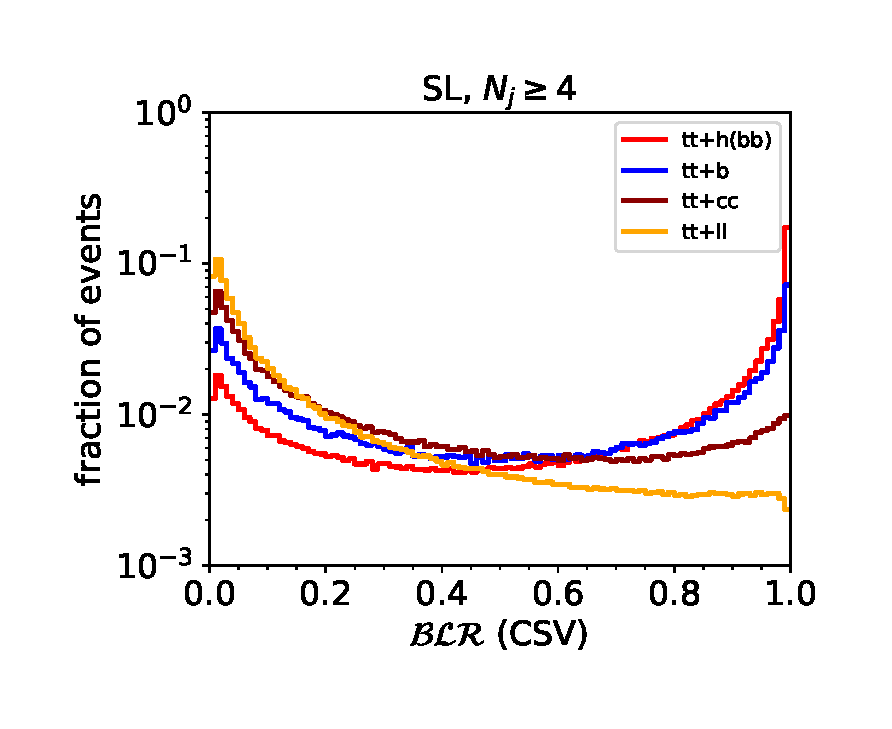
\includegraphics[width=0.5\textwidth]{figures/blr_shape_btagCSV.pdf}} 
\subfloat[Expected performance of the discriminant.]{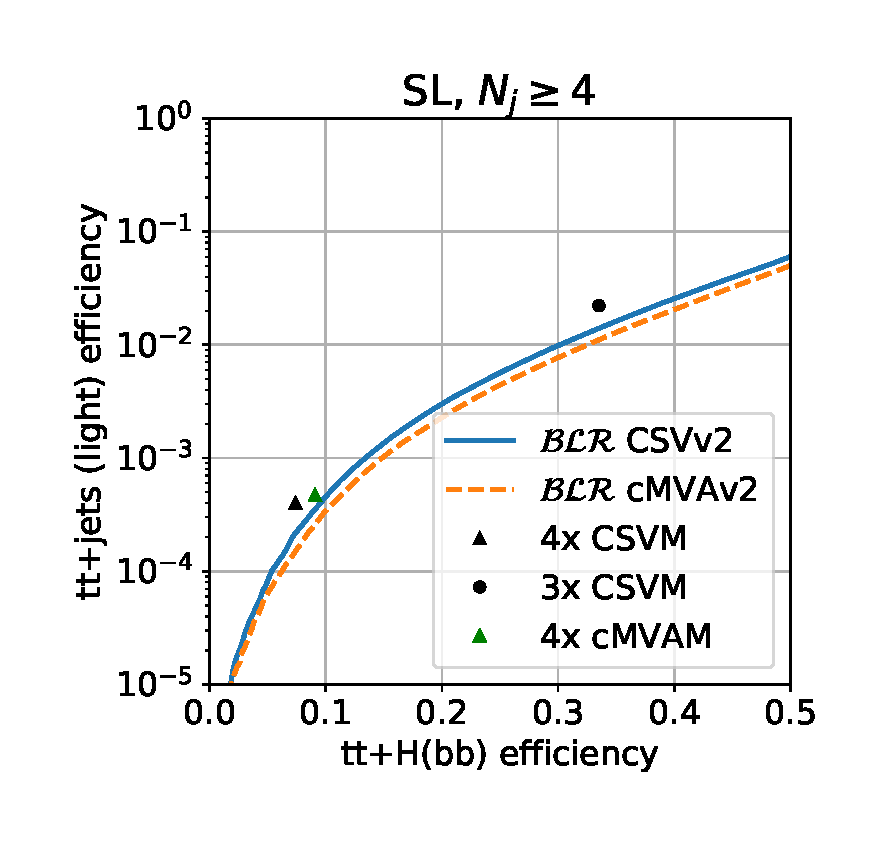
\includegraphics[width=0.5\textwidth]{figures/blr_roc.pdf}}\\
\caption{Simulated distribution and expected performance of $\mathcal{BLR}$ discriminant in the SL channel, requiring at least 4 good jets. On (\textbf{a}), we show the simulated shapes of the discriminant for signal (\ttHbb) and the various \ttbar+jets backgrounds. On (\textbf{b}), we compare the efficiency to select \ttHbb and \ttlf events. We see that the $\mathcal{BLR}$ discriminant compares favorably to a fixed cut on number of b tags. The cMVAv2 discriminator further improves the performance.}
\label{fig:blr_discrimination}
\end{centering}
\end{figure}


\begin{figure}
\begin{centering}
\subfloat[Fraction of events with correct matching.]{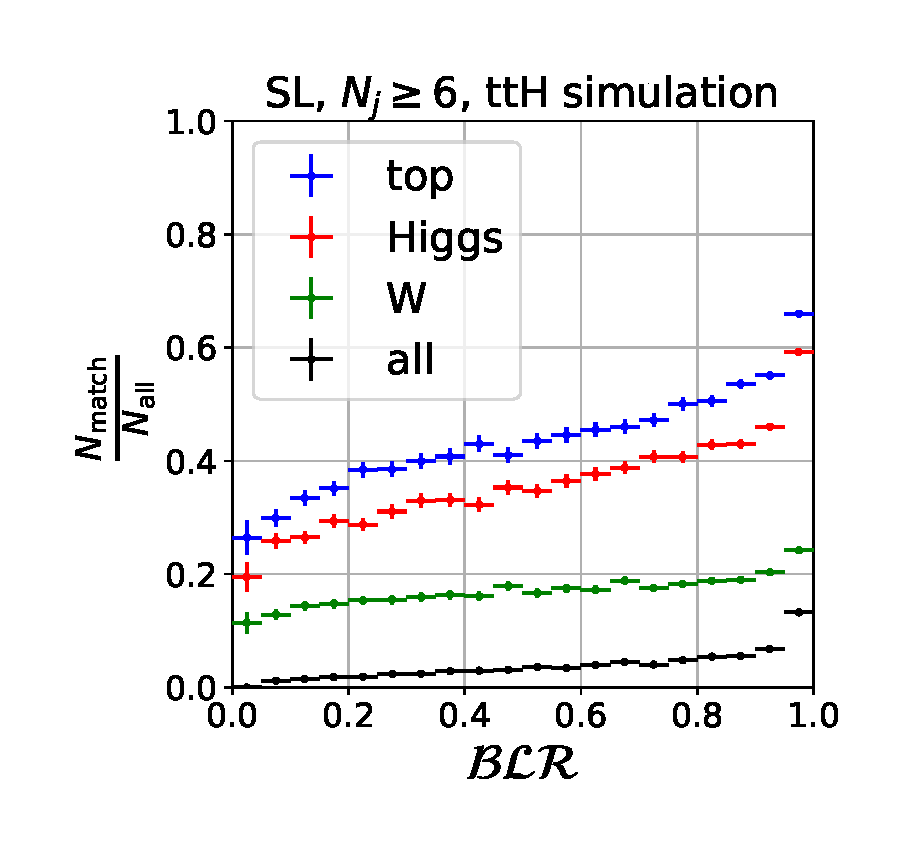
\includegraphics[width=0.5\textwidth]{figures/blr_matching.pdf}} 
\subfloat[Fraction of matched events with correct tagging.]{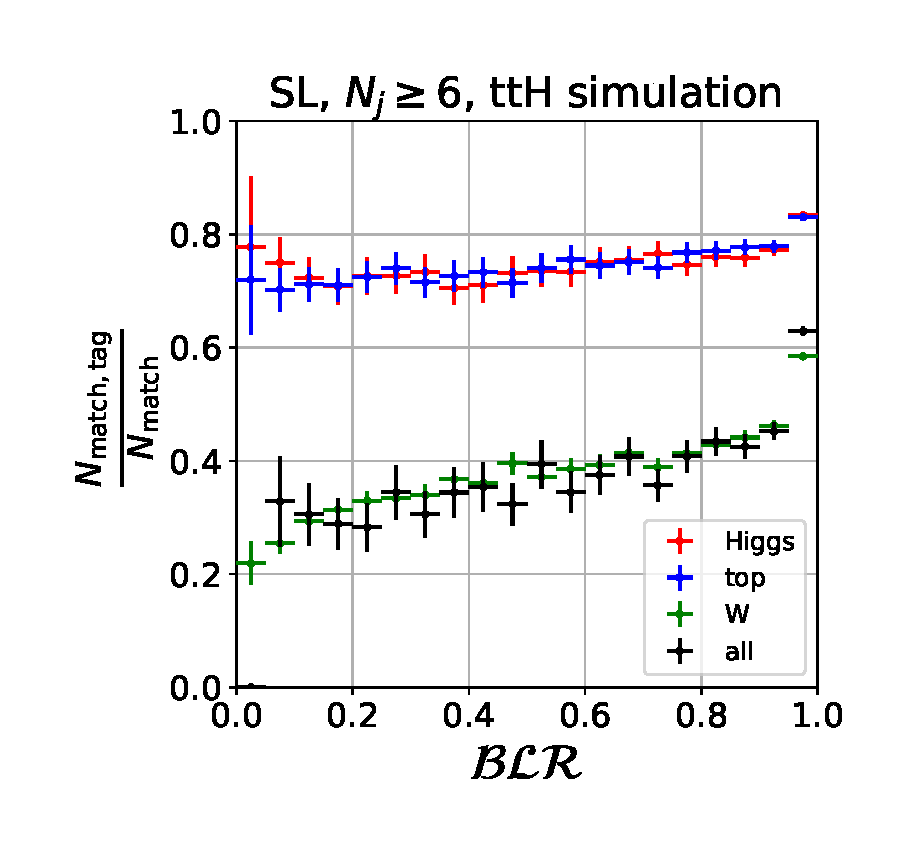
\includegraphics[width=0.5\textwidth]{figures/blr_matching_tag.pdf}}\\
\caption{Estimation of the fraction of events where the bottom quarks from the top quark, the Higgs boson and the light quarks from the W boson are reconstructed as jets in the final state on (\textbf{a}). We study the event-level b tagging efficiency on (\textbf{b}), where we plot the fraction of events where the highest-likelihood permutation correctly assigned the bottom quarks to jets with respect to all events where the quarks were reconstructed as jets without considering tagging.}
\label{fig:blr_matching}
\end{centering}
\end{figure}
 
The likelihood ratio as defined here ignores the differences in $f(\xi_k | \mathrm{b})$ and $f(\xi_k | \mathrm{c})$, meaning that in the case of $\mathrm{W} \rightarrow \mathrm{c}\bar{\mathrm{s}} (\bar{\mathrm{d}})$ decays, the discriminator is inoptimal. We have investigated extending this likelihood to also account for the possibility of such decays by a straightforward extension of $\mathcal{BL}(\vec{\xi} | M\mathrm{b}~1\mathrm{c})$. However, we have found that the additional combinatorial complexity suppresses any increased discrimination power and further progress in this would likely require methods that are better able to deal with the combinatorial problem using kinematic information.

We use this likelihood discriminant to define heavy-flavour enhanced regions, as well as to select the bottom quark candidates in the application of the MEM, as described in \cref{sec:mem_application}. 

As we have used the detailed b tagging discriminator shape information in constructing the $\mathcal{BLR}$, we must experimentally calibrate the full range of this observable using data. This is done by deriving a scale factor between data and simulation that depends on the discriminator value, jet kinematics and flavour using a tag-and-probe method. The tag jet is required to pass the medium operating point that has been described earlier and iteratively correcting the discriminator distribution of the probe jet. In order to extract the weight for the b jets, the procedure relies on dilepton \ttbar events with the contribution from light jets and backgrounds subtracted using simulation, whereas for the scale factor for light jets, Z+jets events are used. The procedure is iterative, as the scale factor for light jets is required for the extraction of the b jet scale factor and vice versa \cite{CMS:2013sea,CMS-PAS-BTV-15-001}. The systematic uncertainties from this reweighting are described in \cref{sec:systematic_unc}.

The leptonic decays of the W boson produce neutrinos, which are only partially reconstructed by the detector as \MET, defined as the negative sum of all the momenta of the reconstructed particles in the transverse plane. In the SL channel, we can directly associate the \MET with the transverse momenta of the neutrinos, through the modelling of the recoil as described in \cref{sec:transfer_functions} whereas in the DL channel, only the total momentum of both neutrinosis  constrained by the \MET.

\subsection{Event selection and categorization}
\label{sec:event_selection}

First, the large multi-jet QCD background is reduced to negligible levels by requiring that at least one of the top quarks in \ttHbb decays leptonically. We divide events to two exclusive lepton categories: SL and DL, based on the multiplicity of the reconstructed charged leptons passing the quality cuts described in \cref{sec:object_id_lep}. This is achieved by vetoing events with any additional leptons passing loosened quality criteria. For the dilepton category, we further suppress the Drell-Yan background by requiring $m_{\ell\ell} > 20\GeV$ and Z+jets by rejecting events with $76\GeV < m_{\ell\ell} < 106\GeV$. Furthermore, the leptons are required to have opposite charge. In the DL same-flavour channels, we require $\MET > 40\GeV$. We do not explicitly distinguish between cases where the top quark decays to $\mathrm{\tau}$ leptons, although these events can still pass the selection in case the $\mathrm{\tau}$ decays leptonically.

Events from \ttHbb have a large number of jets and b tags compared to the V+jets backgrounds. Therefore, we require the presence of at least 4 jets passing the quality criteria (\cref{sec:object_id_jets}), out of which at least 2 must be b tagged according according to the medium working point (\cref{sec:object_id_btag}). This brings us to the \ttbar dominated region, where we further distinguish between 7 categories in the SL channel
\begin{itemize}
\item $\ge 6~\mathrm{jets},\ge 4~\mathrm{b~tags}$; $ 5~\mathrm{jets},\ge 4~\mathrm{b~tags}$; $ 4~\mathrm{jets},4~\mathrm{b~tags}$, that are the most signal-enriched regions,
\item $\ge 6~\mathrm{jets},3~\mathrm{b~tags}$; $5~\mathrm{jets} 3,\mathrm{b~tags}$; $5~\mathrm{jets},3~\mathrm{b~tags}$, that contain a significant amount of \ttcc and \ttbb,
\item $\ge 6~\mathrm{jets},2~\mathrm{b~tags}$, that is \ttlf-enhanced and used to constrain JEC uncertainties,
\end{itemize}
and three categories in the DL channel
\begin{itemize}
\item $\ge 4~\mathrm{jets},\ge 4~\mathrm{b~tags}$,
\item $\ge 4~\mathrm{jets},3~\mathrm{b~tags}$,
\item $ 4~\mathrm{jets},2~\mathrm{b~tags}$,
\end{itemize}
resulting in a total of 10 exclusive categories.

We use the MEM as a \ttHbb to \ttbb discriminator in the categories with $\ge 4$ b tags as these are the primary signal-enriched regions. The categories with 3 b tags ar further subdivided into $\mathcal{BLR} \ge C$ (high) and $\mathcal{BLR} < C$ (low), where the high categories are enriched in \ttHbb and therefore will rely on the MEM for discrimination. The low-$\mathcal{BLR}$ categories are retained as control regions where we fit the jet b tagging discriminator. In the categories with 2 b tags, we fit the jet $p_T$ distribution in order to constrain the jet energy scale correction uncertainties. The value of $C$ is determined so that it would result in a signal acceptance of $\epsilon = 0.5$ and significantly lower background acceptance.

\subsection{Signal extraction}
\label{sec:mem_application}
The likelihood discriminant based on b tagging enhances the \ttbar + heavy flavour component, but the cross-section of \ttbb is still an order of magnitude larger that \ttHbb. Furthermore, we cannot directly reconstruct the resonant peak of the \Hbb~decay as a natural disciminant between the signal and non-resonant background. Even though the width of the SM Higgs boson is relatively small compared to detector resolution ($\Gamma = X~\GeV$), the presence of multiple additional bottom quarks due to top decay in the final state creates a combinatorial self-background in the form of an ambiguity in choosing the candidate jets for the \Hbb~decay.

An experimental mass estimator built from randomly selected jet pairs results in a much broader distribution compared to experimental resolution, whereas choosing the pair of jets that would give a mass closest to $m_H$ would cause also the background to exhibit a signal-like peak.

Therefore, we use the MEM discriminant, introduced in \cref{sec:mem}, to compute theory-motivated weights $P_{\ttHbb}$ and $P_{\ttbb}$ for each candidate event. We construct a discriminant based on the likelihood ratio of these weights,

\begin{equation}
\label{eq:mem_ratio}
P_{\mathrm{s}/\mathrm{b}} = \frac{P_{\ttHbb}}{P_{\ttHbb} + \alpha P_{\ttbb}}
\end{equation} 
which based on the Neyman-Pearson lemma, described in \cref{sec:test_statistic}, is the optimal test statistic between the signal and background hypotheses. The scale factor $\alpha$ is optimized to adjust the relative normalization of the signal and background probabilities and is introduced to allow the dynamic range of $P_{\mathrm{s}/\mathrm{b}}$ to be uniform in the range $P_{\mathrm{s}/\mathrm{b}} \in [0, 1]$. Adjusting this coefficient does not change the signal-to-background discrimination power of the discriminant as it is a monotonic rescaling, but allows us to discretize the distribution into a small number of bins without losing sensitivity.

As an improvement over the search for \ttHbb performed by the CMS experiment in Run I \cite{Khachatryan:2015ila}, we use the MEM discriminant also in categories which are not fully reconstructed, but still contain a large amount of signal, namely 5-jet and 4-jet categories in the SL channel. The details of the additional MEM hypotheses are described in \cref{sec:event_interpretation}. We list the discriminant that has been used in different categories in \cref{tab:cat_discriminant}. 


\begin{table}[h!]
\begin{center}
\caption{The analysis categories and the discriminators used in those categories.}
\label{tab:cat_discriminant}
\begin{tabular}{c|c}
\hline
category & discriminant \\
\hline
SL $\ge6$ jets, $\ge4$ tags & MEM SL $2_{\mathrm{W}} 2_{\mathrm{h}} 2_{\mathrm{t}}$ \\
SL $\ge6$ jets, $3$ tags, $\mathcal{BLR}$ high & MEM SL $2_{\mathrm{W}} 2_{\mathrm{h}} 2_{\mathrm{t}}$ \\
SL $\ge6$ jets, $3$ tags, $\mathcal{BLR}$ low & leading jet b discriminator \\
SL $\ge6$ jets, $2$ tags & leading jet $p_T$ \\
\hline
SL $5$ jets, $\ge4$ tags & MEM SL $1_{\mathrm{W}} 2_{\mathrm{h}} 2_{\mathrm{t}}$ \\
SL $5$ jets, $3$ tags, $\mathcal{BLR}$ high & MEM SL $1_{\mathrm{W}} 2_{\mathrm{h}} 2_{\mathrm{t}}$ \\
SL $5$ jets, $3$ tags, $\mathcal{BLR}$ low & leading jet b discriminator \\
\hline
SL $4$ jets, $\ge4$ tags & MEM SL $0_{\mathrm{W}} 2_{\mathrm{h}} 2_{\mathrm{t}}$ \\
SL $4$ jets, $3$ tags, $\mathcal{BLR}$ high & MEM SL $0_{\mathrm{W}} 2_{\mathrm{h}} 2_{\mathrm{t}}$ \\
SL $4$ jets, $3$ tags, $\mathcal{BLR}$ low & leading jet b discriminator \\
\hline
DL $4$ jets, $\ge4$ tags & MEM DL $2_{\mathrm{h}} 2_{\mathrm{t}}$ \\
DL $4$ jets, $3$ tags, $\mathcal{BLR}$ high & MEM DL $2_{\mathrm{h}} 2_{\mathrm{t}}$ \\
DL $4$ jets, $3$ tags, $\mathcal{BLR}$ low & leading jet b discriminator \\
DL $4$ jets, $2$ tags & leading jet $p_T$ \\
\hline
\hline
\end{tabular}
\end{center}
\end{table}

We use the \ttbb matrix element as a representative background in all cases. This gives the best separation in the most signal-rich categories against \ttbb and is further motivated by simulation, where we see that using this process as background still achieves a high rate of separation in categories enriched in other \ttbar+jets subprocesses. As a future improvement, considering additional background hypotheses in different categories is expected to improve the discrimination at the cost of computational complexity.

As the $\mathcal{BLR}$ method is optimized to identify the set of jets that are most compatible with arising from 4 bottom quarks, we further augment the MEM by assuming that the bottom quarks need to be considered only among those 4 jets, as explained in \cref{sec:event_interpretation}. This means that the we have exactly 4 candidates for the bottom quarks from \Hbb~and $\mathrm{t} \rightarrow \mathrm{W} \mathrm{b}$ decay, whereas the remaining jets are assumed to arise from $\mathrm{W} \rightarrow \mathrm{q} \mathrm{q}'$ or QCD radiation. 

In the next section, we will discuss the systematic uncertainties that affect the analysis.

\subsection{Systematic uncertainties}
\label{sec:systematic_unc}
We have already mentioned in passing that there are a number of experimental as well as theoretical uncertainties that must be taken into account.

Among the experimental uncertainties, the dominant ones are uncertainties on the jet energy scale corrections (\cref{sec:jec_unc}) and the reweighting of the b tagging discriminant (\cref{sec:btag_unc}). Both of these can affect the yields of all the processes, since they change the selection efficiency, as well as the shapes of the final discriminants. In case the source of the uncertainty is the same across several categories, the nuisance parameters associated with the uncertainties are treated as fully correlated.

From the theoretical uncertainties, the most important ones arise from the variation of the renormalization and factorization scale of the \ttbar+jets subprocesses and the \ttH signal. Furthermore, since the \ttbar+jets \texttt{POWHEG} model we currently use in the analysis treats the \ttbb process only at leading order accuracy, where the $\mathrm{b}\bar{\mathrm{b}}$ pair is generated from gluon splittings using a parton shower, we have considerable additional theoretical uncertainties on the modelling of \ttbb.

We give a detailed overview of the most important experimental and theoretical uncertainties along with their estimation in the next sections. The full list of systematic uncertainties along with their effect is show in \cref{tab:systematic_uncertainties}.

\begin{table}[h!]

\begin{center}
\caption{}
\label{tab:systematic_uncertainties}
\begin{tabular}{c|cccc}
\hline
uncertainty & normalization & shape & process & model \\
\hline
JEC (26 sources) & yes & yes & all & gaussian \\
btag & yes & yes & all & gaussian \\
\hline
bla & yes & yes & all & gaussian \\
\hline
\hline
\end{tabular}
\end{center}
\end{table}

\subsubsection{Jet energy correction uncertainties}
\label{sec:jec_unc}
In Run II, we consider various sources of jet energy correction uncertainties with their corresponding correlations, as opposed to a single bulk JEC uncertainty as was done for this analysis in Run I. This significant advancement has resulted from an improved modelling of the detector performance and better calibration techniques developed with more data. 

The magnitude and correlation of the uncertainties on jet energy scale and resolution are estimated in a dedicated CMS analysis and are provided as a vector of per-jet corrections with $p_T$ and $\eta$ dependent correlations. The most important groups of correction uncertainties are the following.
\begin{itemize}
\item Pileup offset, which results from from extra energy deposited in jets from additional pp interactions within the same bunch crossing (in-time pileup) or due to the finite signal decay time in the calorimeters (out-of-time pileup). The uncertainty for this source results from the $\eta$-dependent scale factor used to correct the offset distribution measured in simulation.
\item Relative $\eta$-dependent corrections, which calibrate the forward regions of the detector with respect to the central region. The uncertainties on this source arise from jet energy resolution and from the modelling of ISR+FSR.
\item Uncertainties on the absolute energy scale, which are derived using Z/$\gamma$+jet and multijet data. The energy scale uncertainties are driven by the muon momentum scale and the single pion response in the HCAL. Furthermore, the uncertainties in fragmentation are assessed in a comparison of \texttt{PYTHIA} and \texttt{HERWIG++}.
\item Uncertainties in the modelling of the detector response for jet flavor, which are assessed using simulation and are largest for gluon jets.
\item Finally, due to radiation damage, there is a residual time-dependent uncertainty in the scale corrections, which is estimated using dijet events in different run periods.
\end{itemize}
These 5 groups factorize into about 26 independent sources with up and down variations.

In order to account for the JEC scale uncertainties in the analysis, we propagate the uncertainties in jet energy corrections and resolution to the jet momenta and all the event-level observables that derive from them in MC by shifting the jet energy scale by one standard deviation. This is done separately for all the sources so that we can fully account for the correlations between the various sources. Thus, we are able to account for both the changes in efficiency (normalization) and discriminator shape in the final analysis categories.
In order to propagate the uncertainty to a high-level multivariate observable such as the MEM, we need to recompute it using the variated objects. We use the approximate MEM variation technique of this as described in \cref{sec:mem_uncertainties}.

In addition to uncertainties in the jet energy scale corrections, we also consider uncertainties on the jet energy resolution corrections. 
\subsubsection{B-tagging systematic uncertainties}
\label{sec:btag_unc}
Due to the high number of b tagged jets in the final state, this analysis is sensitive to uncertainties in b tagging. As we have described in \cref{sec:object_id_btag}, we correct for mismodeling in the b tagging discriminator shape using a tag and probe method.

The uncertainties of this correction include the propagation of jet energy scale uncertainty, which affects the determination of the correction through changes in efficiency and the discriminator value. Furthermore, simulation is used to subtract the non-relevant jet flavor components in determining the scale factor for bottom (light) jets. For the scale factor for light jets, the fraction of bottom (charm) jets is variated within 20\% of the MC prediction in the Z+jets simulation used to determine the scale factors. Similarly, for the extraction of the b jet scale factor, the light flavour component in the \ttbar+jets dileptonic sample arises from additional radiation and is estimated to be 20\% \cite{CMS-PAS-BTV-15-001}.

As the b discriminator scale factor is determined in bins of the discriminator value, statistical fluctuations in bins with a low number of data and simulated events introduce an uncertainty on the final scale factor. This uncertainty is only significant in case the size of the fluctuations varies systematically over the b discriminant range. Since the discriminator has a roughly monotonous increasing (decreasing) shape for b jets (light jets), this condition is fulfilled. The statistical uncertainties are accounted for by a sum of polynomials of first and second order, where the nuisance parameter is the overall scale of the distortion.

There is currently no dedicated scale factor for the b discriminator of charm jets, therefore, the uncertainty is conservatively assumed to be twice as large as for the b jet scale factor.

We propagate the uncertainties from b tagging in the form of a set of per-event weights, which are determined from the individual per-jet weights that are used to correct the jet b discriminator distributions.

\fix plot of b-discriminator before and after re-weighting with shape uncertainties.

\subsubsection{Other systematic uncertainties}
We also assess the effect of uncertainties in the lepton identification, isolation and trigger selection, which may have different efficiencies in data and simulation and are thus corrected using scale factors. For muons, we assign a $1\%$ normalization uncertainty for the lepton ID, $1\%$ for isolation and $0.5\%$ for the so-called HIP effect, on top of the statistical uncertainties on the muon scale factor\cite{CMS:2017_mu_sf}. For electrons, we use $p_T$ and supercluster $\eta$-dependent scale factor uncertainties derived using a tag-and-probe method, which are generally below $1\%$ \cite{CMS:2017_ele_sf}.

As the pileup profile in simulation is corrected to data using a pileup-dependent scale factor, we estimate the uncertainty in the pileup correction by varying the minimum bias cross section from $\sigma = 69.2$~mb by $4.6\%$, corresponding to the uncertainty in the number of interactions in minimum bias events from luminosity and cross section\cite{CMS:2017_pu_weight_twiki}.

Furthermore, the uncertainty on total integrated luminosity is estimated to be $2.5\%$ using cluster counting in the pixel detector and affects all processes\cite{CMS:2017sdi,CMS:2017_lumi}.

\subsubsection{Theoretical uncertainties}
The most important theoretical uncertainties arise from the \ttbar+heavy flavour processes, namely \ttbb, \tttwob, \ttb~and \ttcc. Currently, there is no direct way to determine these backgrounds directly from data. Therefore, we assign a conservative 50\% normalization uncertainty on all the \ttbar+heavy flavour processes, uncorrelated across the aforementioned subprocesses.

The cross sections of all involved signal and background processes are known to at least NLO accuracy, with uncertainties estimated through PDF QCD renormalization and factorization scale variations on the \ttbar~background. Furthermore, we use dedicated MC simulation to estimate the effect of the renormalization and factorization scales and the initial and final state radiation on the final discriminant shape. Shape uncertainties from PDF variations are found to be negligible and thus not considered further in the analysis.

\subsection{Statistical method}
\label{sec:statistical_method}
In order to interpret the data, we use the same statistical framework as has been used for other Higgs boson searches in the CMS collaboration\cite{Chatrchyan:2012xdj,Chatrchyan:2012tx,ATLAS:2011tau}. We wish to measure the signal strength modifier $\mu = \sigma_{\ttH}/\sigma_{\ttH,\mathrm{SM}}$ and in the absence of an observed signal, exclude $\mu \ge \mu^{CL}$ at a certain confidence level. The null hypothesis ($H_0$) is therefore the presence signal with a given $\mu$ and background, whereas the alternative hypothesis is no signal ($H_1, \mu = 0 $). Based on the data, we seek to exclude the null hypothesis above a certain $\mu$.

The predictions for both signal (denoted as $s$) and background (denoted as $b$) yields are subject to uncertainties introduced in \cref{sec:systematic_unc} such that the expectations are functions of the nuisance parameters $\theta$: $s(\theta)$ and $b(\theta)$. The uncertainties are assumed to be either fully correlated or uncorrelated, as is more appropriate and conservative, which allows the likelihood function to be written in a factorized form.

To determine confidence intervals on the Higgs boson production cross section and thus quantify the absence of a signal, we use the $CL_s$ method \cite{Junk:1999kv,Read:2002}, which defines the likelihood function $\mathcal{L}(\mathrm{data} | \mu, \theta)$ as

\begin{align}
\label{eq:likelihood}
\mathcal{L}(\mathrm{data} | \mu, \theta) =&  \mathrm{Poisson}(\mathrm{data} | \mu \cdot s(\theta) + b(\theta)) \cdot p(\tilde{\theta} | \theta)\\
=& \prod_{i\in \mathrm{bins}} \frac{(\mu s_i + b_i)^{n_i}}{n_i!} \exp{[-(\mu s_i + b_i)]} \cdot p(\tilde{\theta} | \theta).
\end{align}
We have used Poisson probabilities to observe $n_i$ events in the bin $i$ of a discretized distribution, given an expectation $\mu s_i + b_i$. The distribution $p(\tilde{\theta} | \theta)$ encodes the prior knowledge on the nuisance parameters, which have default values $\tilde{\theta}$. This likelihood function can be computed both with observed data and with "pseudodata", which is constructed from simulation under a specific hypothesis.

We use the test statistic $\tilde{q}_\mu$, based on the profile likelihood ratio\cite{Cowan:2010js}, to assess the compatibility of the data with either the \textit{background-only} or \textit{signal+background} hypotheses:

\begin{equation}
\tilde{q}_\mu = -2 \ln{\frac{\mathcal{L}(\mathrm{data} | \mu, \hat{\theta}_\mu)}{\mathcal{L}(\mathrm{data} | \hat{\mu}, \hat{\theta})}},\ 0 \le \hat{\mu} \le \mu.
\end{equation}
This test statistic is constructed such that it considers only models with $\mu \ge 0$, futhermore it is constrained to be one sided by $\hat{\mu} \le \mu$ such that data with $\hat{\mu} > \mu$ are not used as part of the rejection region for the test on the upper limit of $\mu$.

Here $\hat{\mu}_\theta$ is the conditional maximum likelihood estimator of $\theta$ given a fixed value $\mu$, wheras $\hat{\mu}$ and $\hat{\theta}$ refer to the overall maximum likelihood estimators of both quantities. For a given signal strength modifier $\mu$ that we test, we first find the observed value of $\tilde{q}_\mu^{\mathrm{obs}}$ and the nuisance parameters $\hat{\theta}_0$ (background hypothesis) and $\hat{\theta}_\mu$ (signal hypothesis). Then, in order to compute the $CL_s(\mu)$, we compute the p-values of the signal and background hypotheses using

\begin{equation}
p_{\mu} = \int_{\tilde{q}_{\mu}{\mathrm{obs}}}^\infty f(\tilde{q}_{\mu} | \mu, \hat{\theta}_{\mu})\ \mathrm{d}\tilde{q}_\mu
\end{equation}
and

\begin{equation}
1 - p_b = \int_{\tilde{q}_{\mu}^{\mathrm{obs}}}^\infty f(\tilde{q}_{\mu} | 0, \hat{\theta}_0)\ \mathrm{d}\tilde{q}_{\mu}.
\end{equation}

The p-values are the probabilities of observing results as extreme or more given the underlying hypothesis and are derived from the probability densities of $\tilde{q}_{\mu}$ under a given hypothesis: $f(\tilde{q}_\mu | \mu, \hat{\theta}_\mu^{\mathrm{obs}})$. We find the 95\% confidence level on the upper limit of $\mu$ by adjusting $\mu$ until

\begin{equation}
\mathrm{CL}_s(\mu) = \frac{p_\mu}{1 - p_b} < 0.05.
\end{equation}
Alternatively, if $\mathrm{CL}_s < \alpha$ at $\mu$, then the Higgs boson is excluded at a production rate of $\mu$ or higher with a confidence level $1 - \alpha$.

In order to compute the upper limit on $\mu$ given the observed data, we need the PDFs $f(\tilde{q}_\mu | \mu, \hat{\theta}_\mu^{\mathrm{obs}})$, which can be derived using a Monte Carlo method by generating pseudo-data assuming the given signal strength $\mu$ and fitting the observed data to evaluate the test statistic. As the MC procedure for generating the PDFs can be very time consuming, we use an approximate asymptotic distribution \cite{Cowan:2010js} for the PDF $\tilde{q}_\mu$, which results from the Wald approximation \cite{wald1943tests}:

\begin{equation}
-2 \ln{\lambda(\mu)} = \frac{(\mu - \hat{\mu})^2}{\sigma^2}+ \mathcal{O}(1/\sqrt{N})
\end{equation}
where $\sigma$ is the standard deviation of $\hat{\mu}$ derived from the full covariance matrix of the likelihood function.

Using the asymptotic distribution for $f(\tilde{q}_\mu | \mu, \hat{\theta}_\mu^{\mathrm{obs}})$, we find the upper limit for $\mu$ at a confidence level of $1 - \alpha$ to be

\begin{equation}
\mu = \hat{\mu} + \sigma \Phi^{-1}(1 - \alpha)
\end{equation}
where $\Phi^{-1}$ is the inverse of the cumulative distribution of the Gaussian PDF. The standard deviation of $\mu$ can be computed from the likelihood function \cref{eq:likelihood} using the so-called Asimov data set, where the MC prediction is used for $s_i$ and $b_i$.

We will also quote the expected sensitivity of the measurement, which is derived from simulation, assuming $\mu = 1$ and computing the median expected upper limit on $\mu$ using the asymptotic formulae. 

\subsubsection{Uncertainties in the statistical model}

Our prior knowledge of the systematic uncertainties is encoded in $p(\tilde{\theta} | \theta)$, where the nuisance parameters $\theta$ are minimized in the profile likelihood method in a frequentist sense. We use $\tilde{\theta}$ to represent our best estimate of the nuisance parameters, which can be
\begin{itemize}
\item gaussian, used for shape variations,
\item log-normal used for nuisances that do not have physical negative values,
\item flat, in case we cannot assign a prior uncertainty.
\end{itemize}

We use the Barlow-Beeston method in the fit to account for limited number of simulation events. In this method, the number of predicted events for a background component in a binned distribution is added as a nuisance parameter in the likelihood and minimized with the initial values arising from the observed Poisson counts using Newton's method \cite{Barlow:1993dm}. 

\subsubsection{Analysis of the model}
In this section, we will study the expected sensitivity predicted by the statistical model. We will look in detail at the effect of systematic uncertainties in the form of the constraints on the nuisance parameters after having been fit to pseudo-data derived from MC.

\subsection{Results}
After having validated the statistical model on simulation, we include data in a step-by-step fashion by unblinding the data in the various control regions successively.


\newpage
\printbibliography

\end{document}